%% The following is a directive for TeXShop to indicate the main file
%%!TEX root = diss.tex

\chapter{An Interpretation of 3D Reconstruction}
\label{ch:3DRecon_Interp}
In Chapter~\ref{ch:3DRecon_Mapping}, we have established a mapping from a well defined problem space to a suite of algorithms through evaluating the performance under synthetic situations. However, the claim that this mapping is useful in terms of helping users find the best possible algorithm given problem conditions, or easing the use of complicated vision algorithm, is still unclear. Thus a thorough evaluation is needed to answer those questions.

However, such an evaluation faces several challenges: 1). the derived mapping doesn't pose strict constraints on the type of material and geometry, thus the evaluation should target a vast amount of objects to reach a solid conclusion, which is obvious not a practical approach; 2). the sense of ease of use is a fairly objective measure, the typical method is conduct user experiments. However, user studies is also limited that it only tests the performance for a small set of algorithms and a small set of conditions. Without covering a large range of possiblities, the results would be biased or even wrong. For instance, ???. Thus a new approach is needed to measure the complexity of the traditional the newly proposed way of reconstructing an object, which should be independent to problem space and selected algorithms.

% In order to validate the 3D reconstruction mapping derived from Chapter~\ref{ch:3DRecon_Mapping}, evaluation of the object centric model into appropriate solutions must be shown. Our interpreter is based on the direct evaluation of the performance of each 3D reconstruction algorithm under different conditions presented in Chapter~\ref{ch:3DRecon_Mapping}. From this analysis of how algorithms perform on objects which have different visual and geometric properties, an algorithm(s) can be definitively chosen based on which performed best on the training images.

% The three algorithms introduced in our test bench are: the PMVS proposed by \citeauthor{furukawa2010accurate}, the example-based Photometric Stereo proposed by \citeauthor{hertzmann2005example}, and a standard gray-coded Structured Light technique with error rejection.

Although only three algorithms selected, all of which are the top performers in the corresponding field, thus are sufficient to demonstrate the framework's ability to translate the descriptive model into a reconstruction. Furthermore, the integration of a new algorithm requires the same process preseneted in Chapter~\ref{ch:3DRecon_Mapping}, allowing researchers to contribute novel algorithms to the framework.

\section{Evaluation Methodology}
To prove that the proposed mapping from a condition to an algorithm is a valid one, we need to construct a rigorous evaluation method. In this section, we deal with the steps that are involved to validate the mapping, and the underlying theory to support it.

\subsection{Objective}
% [Develop a description (or access an existing version) of what is to be evaluated and how it is understood to work.]
This evaluation intends to test the effectiveness and robustness of the derived mapping in Chapter~\ref{ch:3DRecon_Mapping}.

% \subsection{Frame}
% Set the parameters of the evaluation its purposes, key evaluation questions and the criteria and standards to be used.

% \subsubsection{Purpose}
% [What are the primary purposes and intended uses of the evaluation?]
% The evaluation intends to find out that the derived mapping can indeed find the algorithm that produces the best possible result from a suite of algorithms.

\subsection{Key Evaluation Questions and Steps}
% [What are the high level questions the evaluation will seek to answer? How can these be developed?]

The most important questions we should always ask when coming up with something new is: 1). \textit{does the proposed framework work?}; 2). \textit{is it an improvement to previous method?}. To put it more formally, the two key questions we need to address or evaluate for the derived mapping is

\subsubsection{1. Effectiveness: Does the mapping return the best-possible result?}
Given a correct description of the object, the algorithm chosen by the mapping should give the best reconstruction result. We use both synthetic and real-world data to test if this is indeed true. For the synthetic data, the quantitative result is possible due to the ground truth. However, the quantitative results are not available for real-world data since we don't have the groundtruth. We use the same quantitative metrics used in Chapter~\ref{ch:3DRecon_Mapping}. Therefore, visual analysis is utilized for real-world objects. We use the quantitative measure from Chapter~\ref{ch:3DRecon_Mapping}.

The evaluation steps are:
\begin{itemize}
\item Data collection: the synthetic data is generated by the Blender using the same setups in Chpater~\ref{ch:3DRecon_Mapping}. The real-world data are captured using different setups: for MVS, a Nikon D700 camera with [focal] lens are used; for photometric images, a Nikon D700 camera with [focal] lens, and a handheld lamp are used; for structured light images, a Nikon 700 camera and a [??] projector are used.
\item Synthetic data: since the ground truth is available, we need to compare both the quantitative results and qualitative results to the result from the mapping to see if they are consistent.
\item Real-world data: since the ground truth is not available, we only visually analyse the quality of the reconstruction and see if it's consistent with the mapping.
\end{itemize}

% \subsubsection{2. Usefulness of Mapping: How the mapping will return the result based on your description and your requirements}
% The purpose of the framework is not to compare which algorithm gives the best result, but to get the best possible reconstruction result given the correct description. Therefore, we want to see how well it works given the correct description, and how badly the result deteriorates given the incorrect description.

% The evaluation steps are:
% \begin{itemize}
% \item We chose three objects so that each algorithm would be activated by the mapping once as a demonstrative result.
% \item 
% \end{itemize}

% \subsubsection{2. Robustness: Does the mapping still return the best algorithm given an incorrect description?}
% Assume given a incorrect description of the object, will the mapping return a less satisfactory result instead, which is what it should behave like?

% \subsubsection{3. Improvement: Is the mapping more useful than the traditional approach?}
% Aside from being able to get the correct results, it's also important that the proposed approach has significant advantages over the traditional ones. We first need to identify the traditional way of employing reconstruction algorithms, find out the strengths and weakness and see if the proposed approach is superior than the exising one in the claimed aspects. The following are the aspects we set out to compare:
% \begin{itemize}
% \item is it easier?
% \item does it cater to more general object?
% \end{itemize}

% The evaluation steps are:
% \begin{itemize}
% \item Define the fundamental steps for both the traditional approach and the one proposed in the thesis.
% \item we adopt the same approach for analysing algorithmic complexity, and use basic step as the unit step to evaluate the complexity of using these two approaches. Complexity analysis is also a tool that allows us to explain how an algorithm behaves as the input grows larger. fundamental instructions/steps
% \end{itemize}

% \subsubsection{Criteria}
% Determine what `success' look like? What should be the criteria and standards for judging performance? Whose criteria and standards matter? What process should be used to develop agreement about these?

% \subsubsection{Steps}
% [Collect and retrieve data to answer descriptive questions about the activities of the project/programme/policy, the various results it has had, and the context in which it has been implemented.]

\section{Parameter Setting}
We provide results from three different descriptios where wach activates a different algorithm and provides a demonstrative result.
To address if the derived mapping works, The first step of the process is to estimate the amount of property in the object. We use a try-and-fit approach, where the user change the value of each property and see if the rendered result looks alike the real object. A similar approach can be found in the~\cite{Berkiten:2016:ARB} where the author also used a synthetic dataset to find the contributing factors of PS.
\begin{figure}[!htbp]
\centering
\begin{tabular}{cc}
  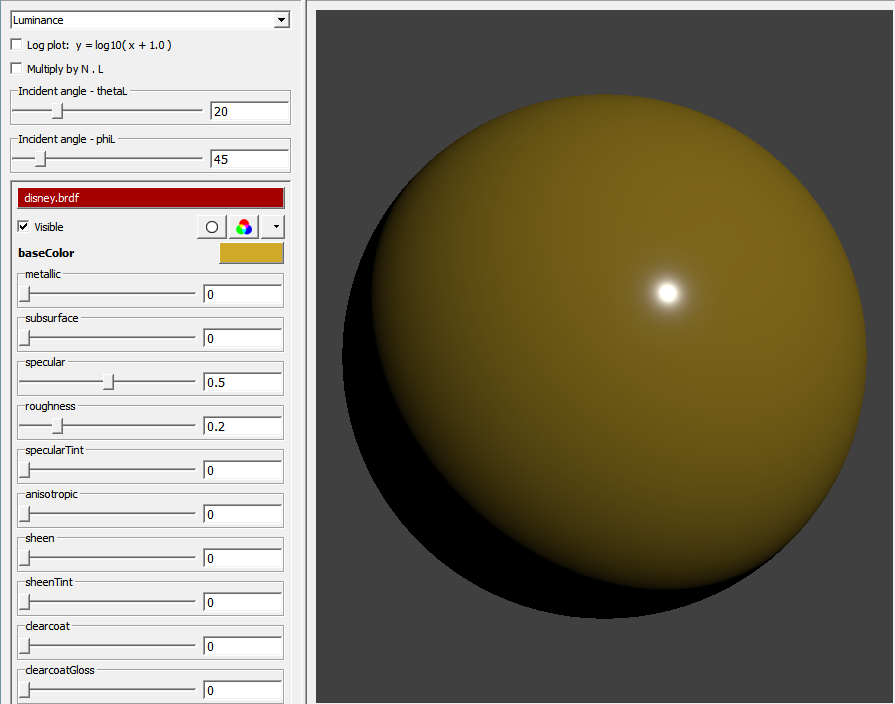
\includegraphics[width=0.5\textwidth]{interp/ui_sphere.PNG}&
  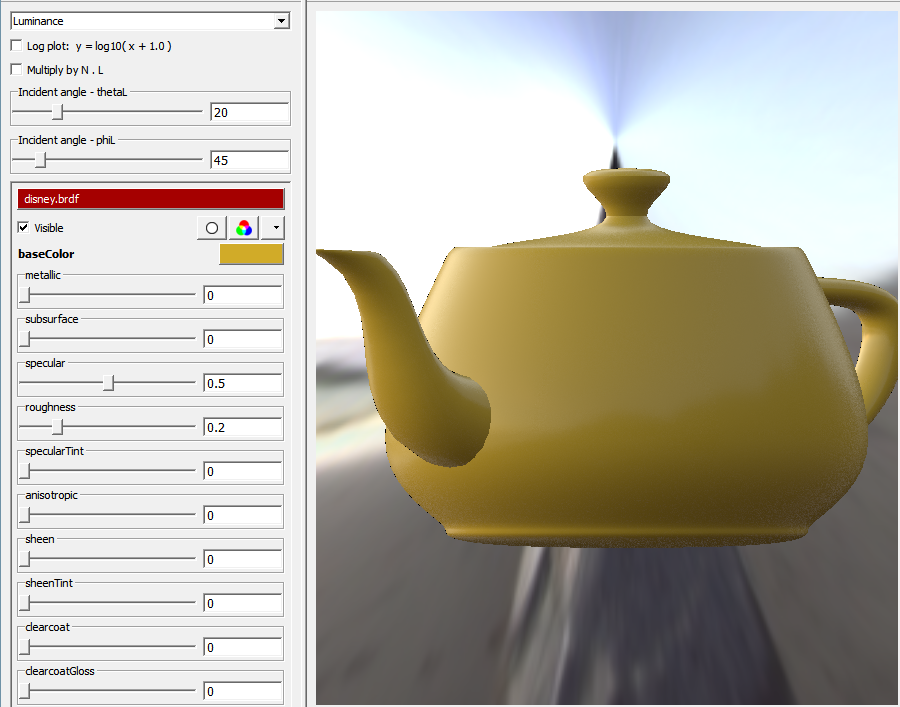
\includegraphics[width=0.5\textwidth]{interp/ui_teapot.PNG}\\
  (a) Lit sphere & (b) Lit teapot\\
\end{tabular}
\caption{The UI of determining the albedo, specular, and roughness of the surface. The albedo is set as around 0.8, which is determined by the value channel of HSV colour. The specular and roughness is set as 0.5, 0.2, respectively. (a) demonstrates the effect of the property setting on a sphere while (b) on a teapot.}
\label{fig:ui}
\end{figure}

\section{Effectiveness of Mapping}
We first evaluate that the derived mapping does what it meant to do: return the best algorithm given a correct description of the object. The idea is that given the description of an arbitrary object, we use all three techniques for reconstruction, and see if the algorithm that has the best quantitative or qualitative result is consistent to the algorithm chosen by the mapping.

\subsection{Synthetic Datasets}
We use one object shown in Figure~\ref{fig:synth_data}, and four property settings in Table~\ref{tab:prop_list_synth_data} to test the validity of the abstraction. Those four settings represents four classes of objects discussed in Chapter~\ref{ch:3DRecon_Desc}. The best suited algorithm as suggested by the mapping derived from Chapter~\ref{ch:3DRecon_Mapping} is included.
\begin{table}[!ht]
  \centering
  \begin{tabular}{l*{5}{c}}
  \hline
  \textbf{Property} & Texture & Albedo & Specular & Roughness & Best-suited techniques\\
  \hline
  (a) & 0.2 & 0.8 & 0.2 & 0.8 & PS, SL\\
  (b) & 0.2 & 0.8 & 0.5 & 0.2 & PS, SL\\
  (c) & 0.8 & 0.8 & 0.2 & 0.8 & MVS, PS, SL\\
  (d) & 0.8 & 0.8 & 0.5 & 0.2 & MVS, PS, SL\\
  \hline
  \end{tabular}
  \caption{Property lists of the test objects.}
  \label{tab:prop_list_synth_data}
\end{table}

\begin{figure}[!htbp]
\centering
\begin{tabular}{cc}
  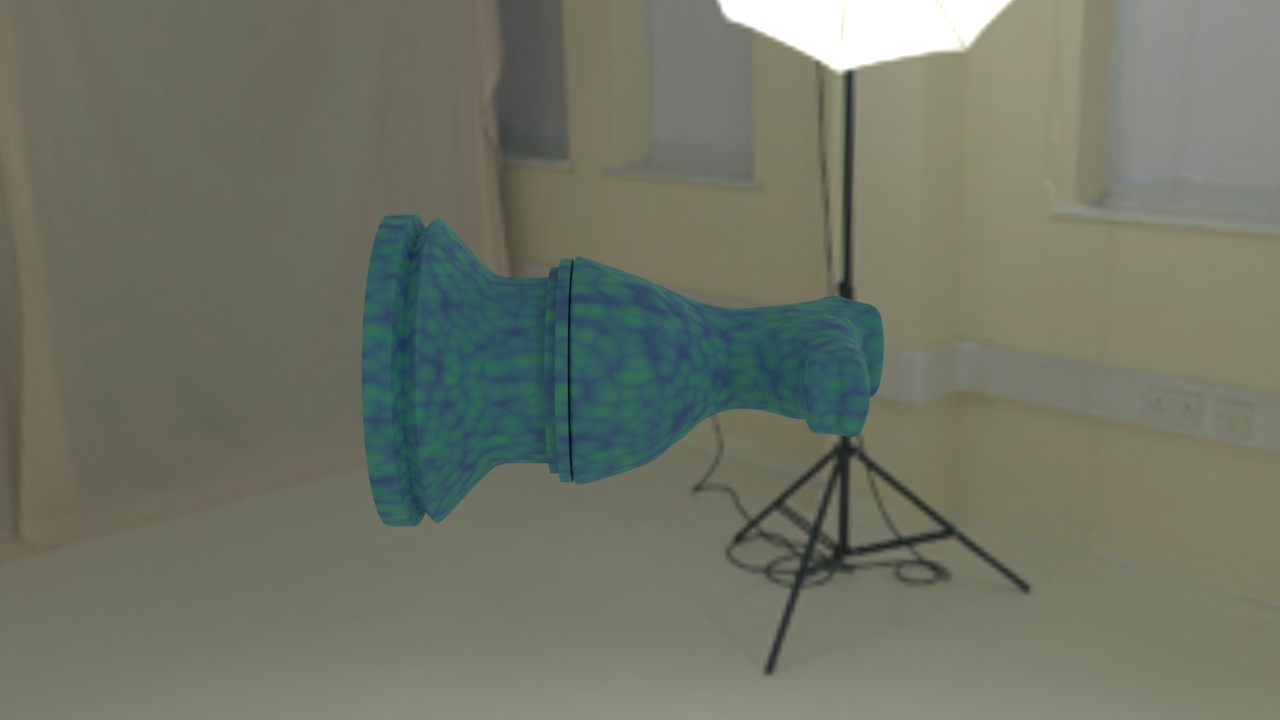
\includegraphics[width=0.33\textwidth]{interp/synth_data/knight/knight_mvs}&
  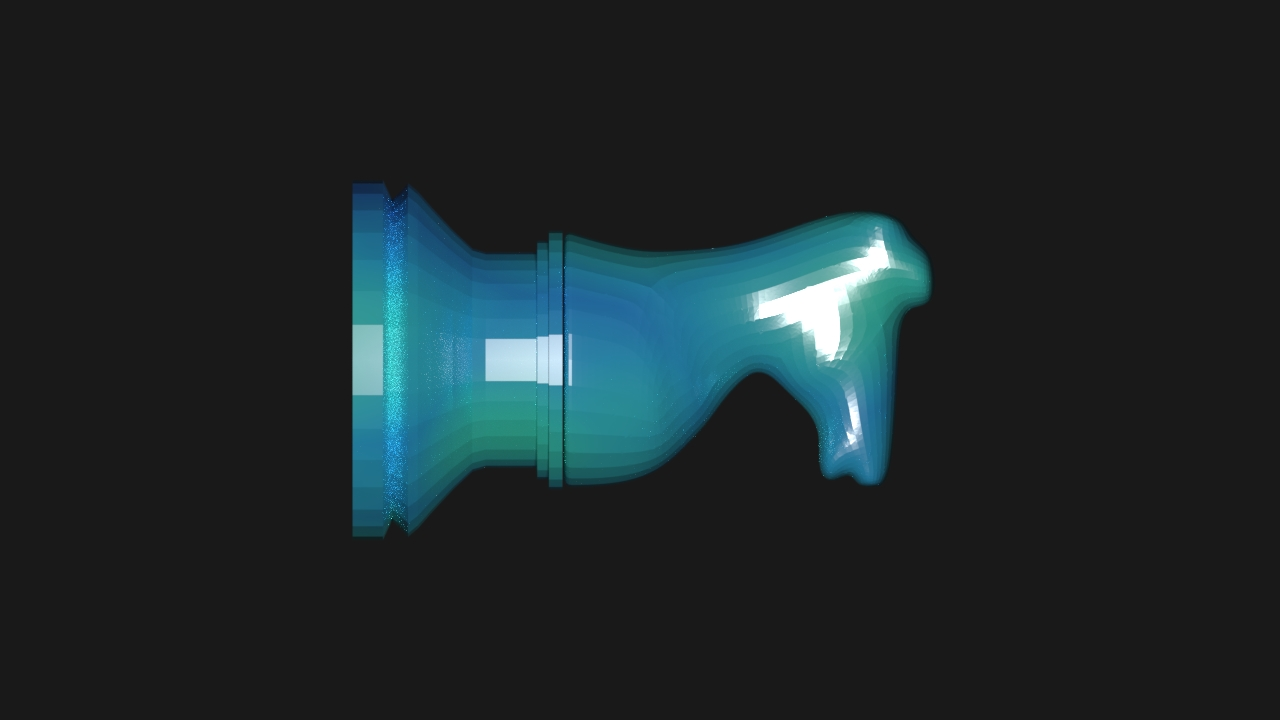
\includegraphics[width=0.33\textwidth]{interp/synth_data/knight/knight_ps}\\
  MVS & PS\\
  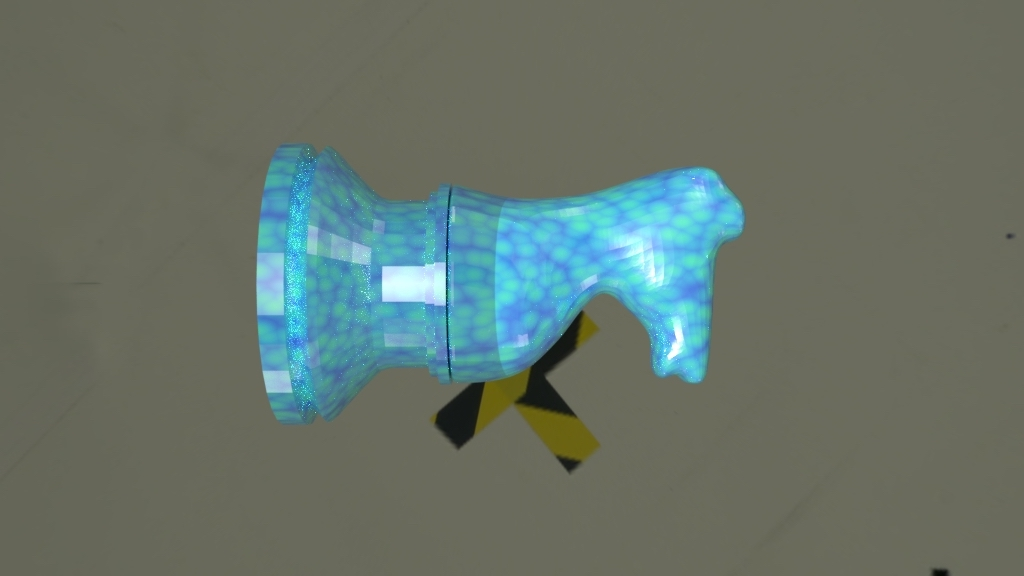
\includegraphics[width=0.33\textwidth]{interp/synth_data/knight/knight_sl}&
  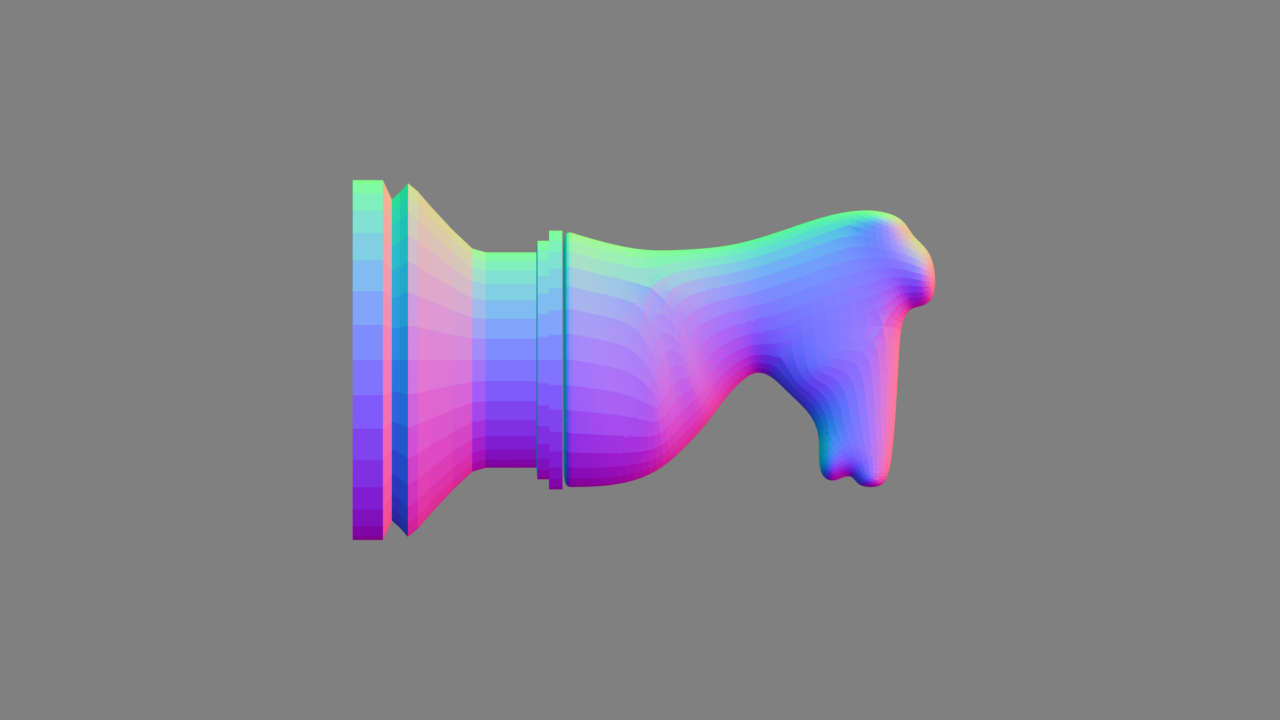
\includegraphics[width=0.33\textwidth]{interp/synth_data/knight/knight_ps_gt}\\
  SL & Normal groundtruth\\
\end{tabular}
\caption{The synthetic datasets and groundtruth for the evaluation}
\label{fig:synth_data}
\end{figure}

% Here is the Table to test the effectiveness of the mapping
% \begin{figure}[!htbp]
% \centering
% \begin{tabular}{cccccc}
% \hline
% & & Mapping & \multicolumn{2}{c}{Accu\&Cmplt} & Norm\\
% \hline
% \multirow{2}{*}{Obj} & \multirow{2}{*}{Desc} & \multirow{2}{*}{Algo} & PMVS & Gray SL & Example PS\\
% 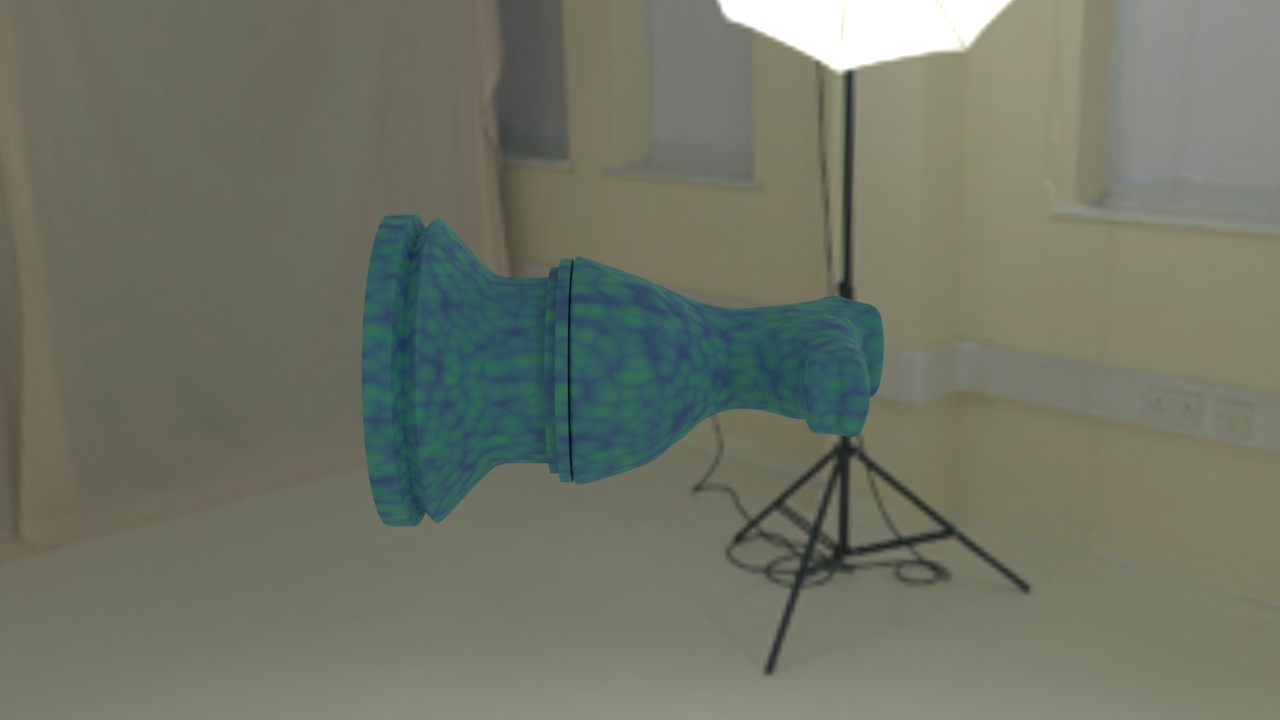
\includegraphics[width=0.15\textwidth]{interp/synth_data/knight/knight_mvs} &
% 02080208 & EPS, GSL & 
% 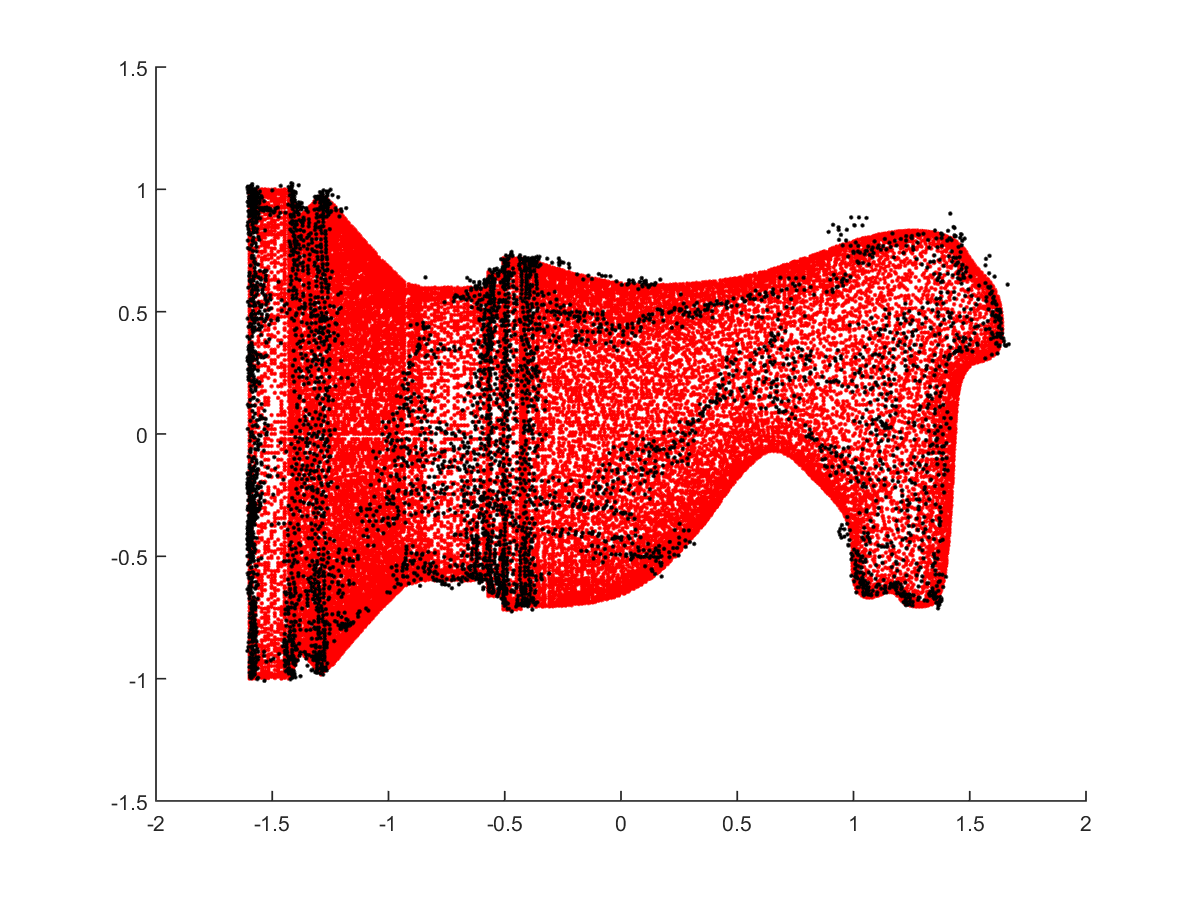
\includegraphics[width=0.15\textwidth]{interp/synth_data/knight/knight_mvs_02080208} &
% 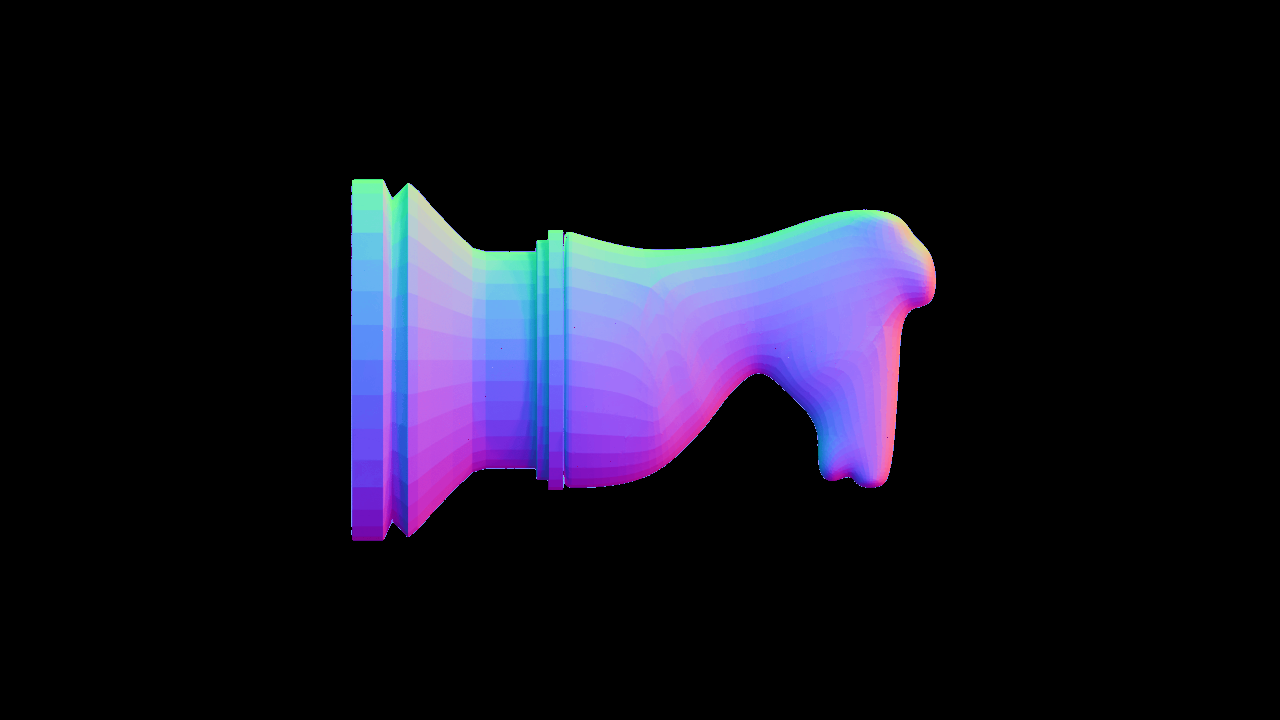
\includegraphics[width=0.15\textwidth]{interp/synth_data/knight/knight_ps_02080208} &
% 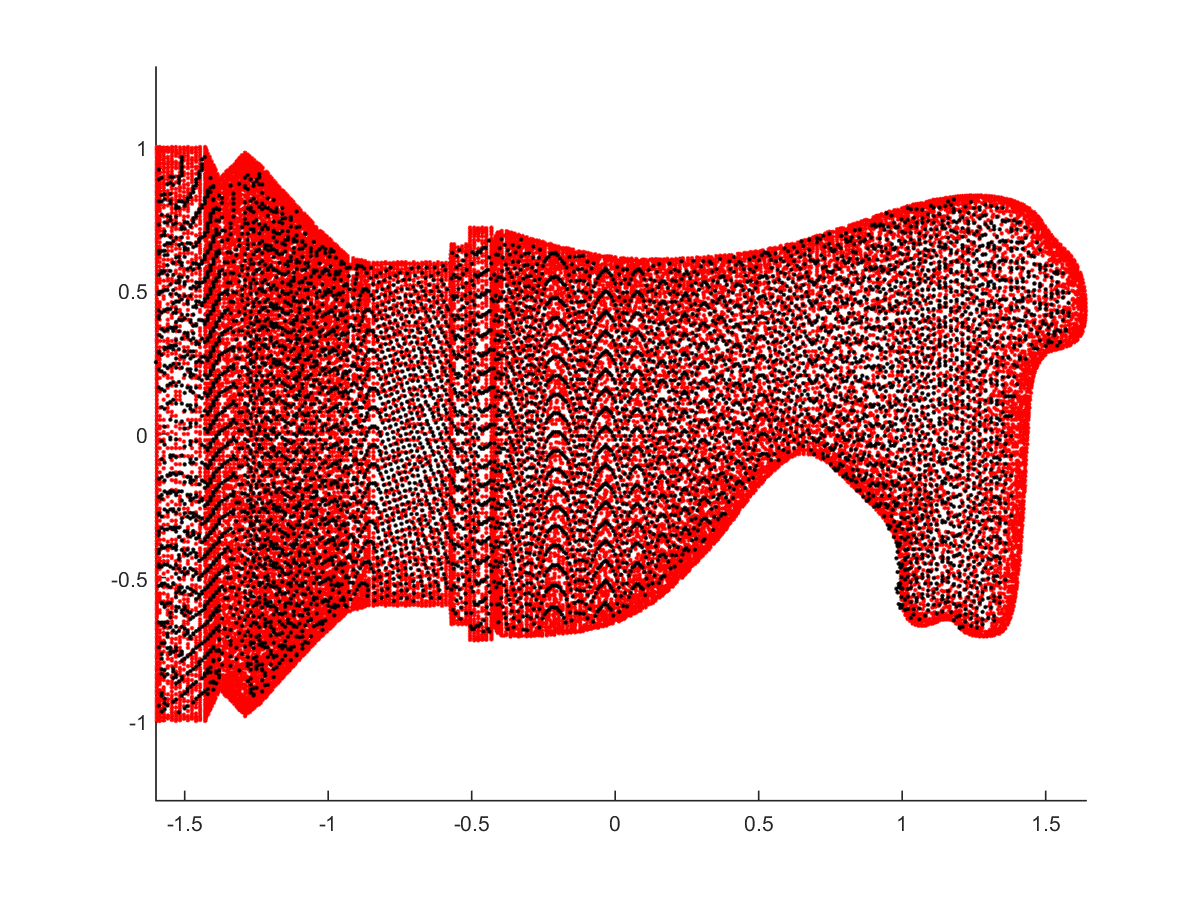
\includegraphics[width=0.15\textwidth]{interp/synth_data/knight/knight_sl_02080208}\\
% \hline
% \end{tabular}
% \end{figure}

Now we show both the quantitative results and qualitative results of the test objects, and see if the results is consistent with the techniques selected by our abstraction. The result is shown in Figure~\ref{fig:synth_data_results}.
\begin{sidewaysfigure}[!htbp]
\centering
\begin{tabular}{c|ccccc}
  Mapping & Quantitative results & ~ & Qualitative results & ~\\
  \hline
  PS, SL & 
  \includegraphics[width=0.2\textwidth]{interp/synth_data/knight/knight_02080208}&
  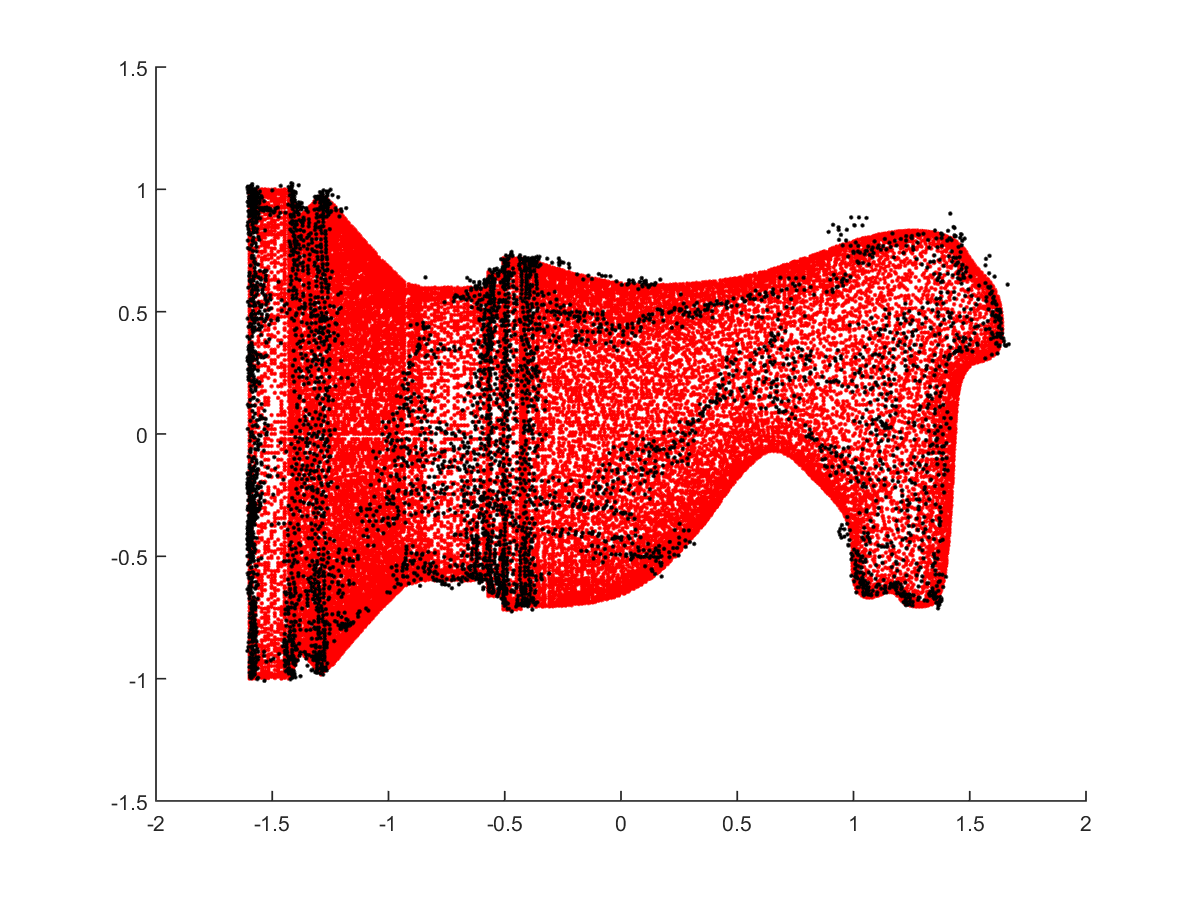
\includegraphics[width=0.2\textwidth]{interp/synth_data/knight/knight_mvs_02080208.png}&
  \fcolorbox{red}{white}{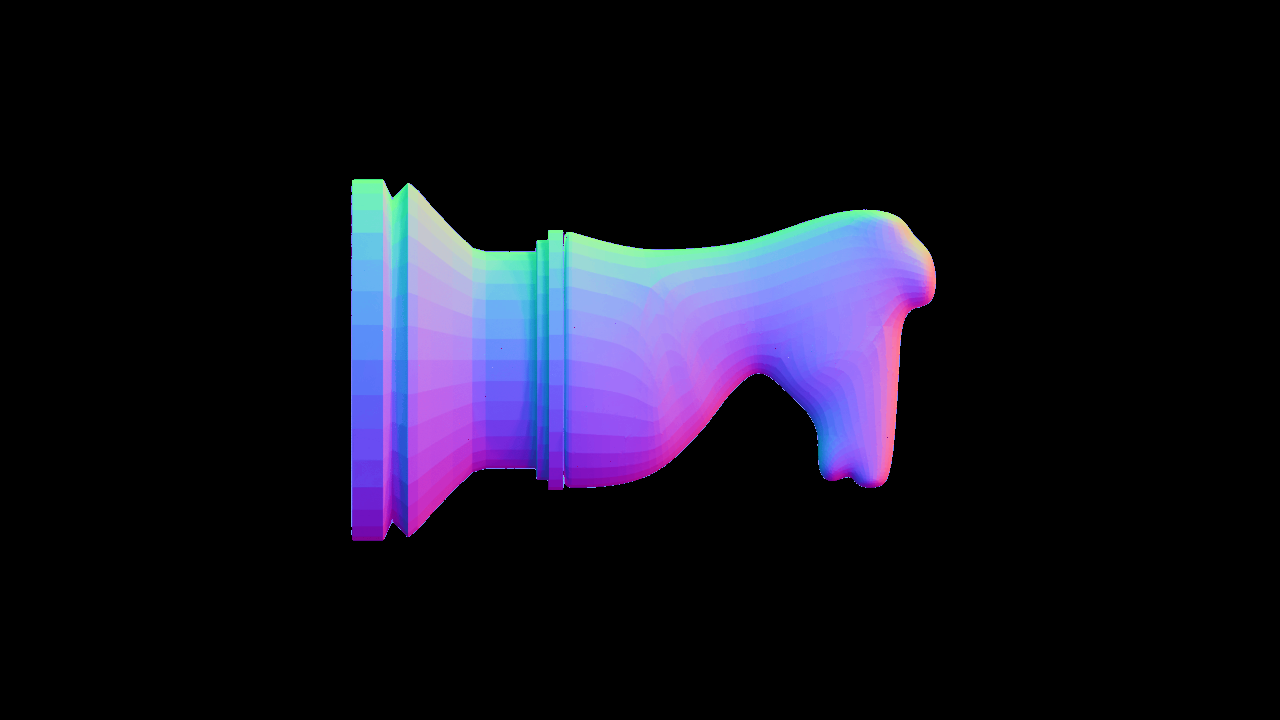
\includegraphics[width=0.2\textwidth]{interp/synth_data/knight/knight_ps_02080208.png}}&
  \fcolorbox{red}{white}{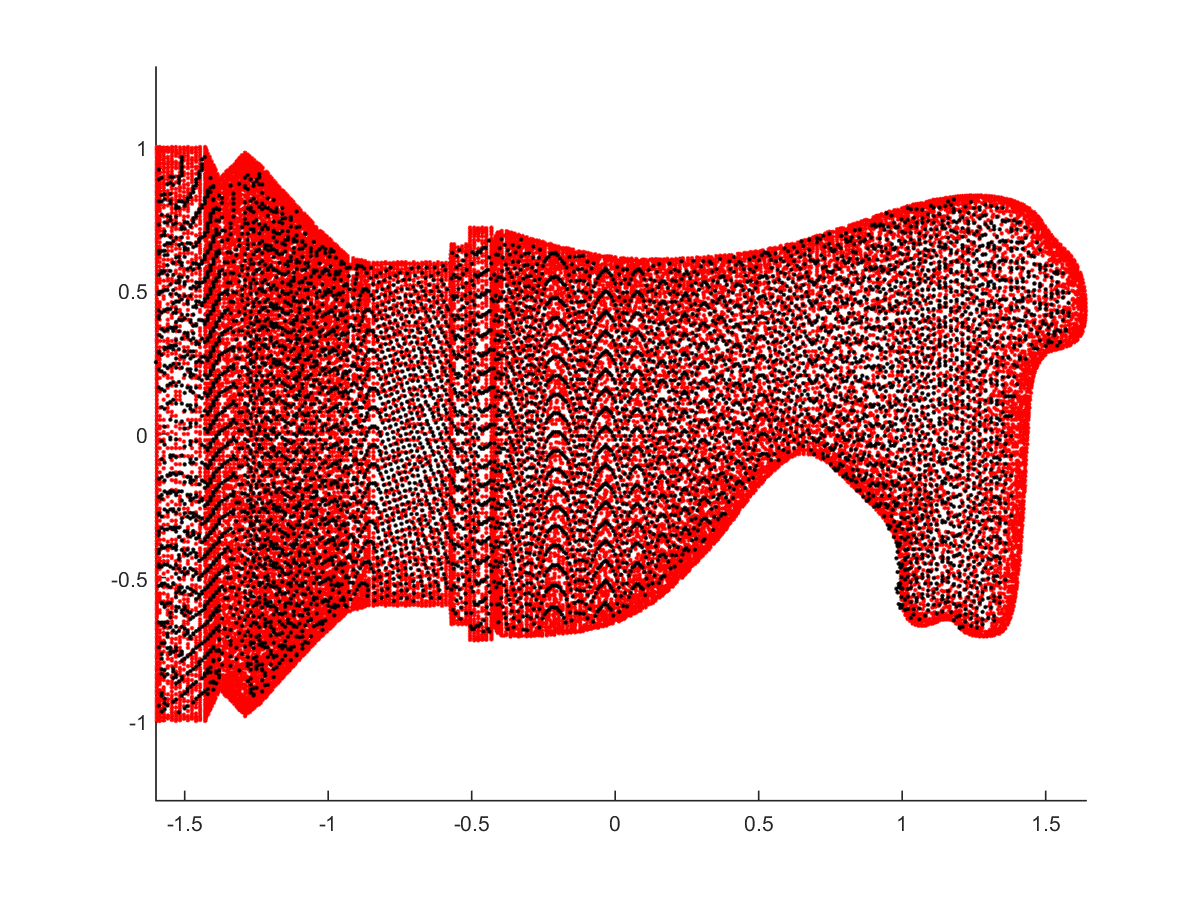
\includegraphics[width=0.2\textwidth]{interp/synth_data/knight/knight_sl_02080208.png}}\\
  & \multicolumn{4}{c}{(a). tex(0.2), alb(0.8), spec(0.2), rough(0.8)}\\
  PS, SL &
  \includegraphics[width=0.2\textwidth]{interp/synth_data/knight/knight_02080502}&
  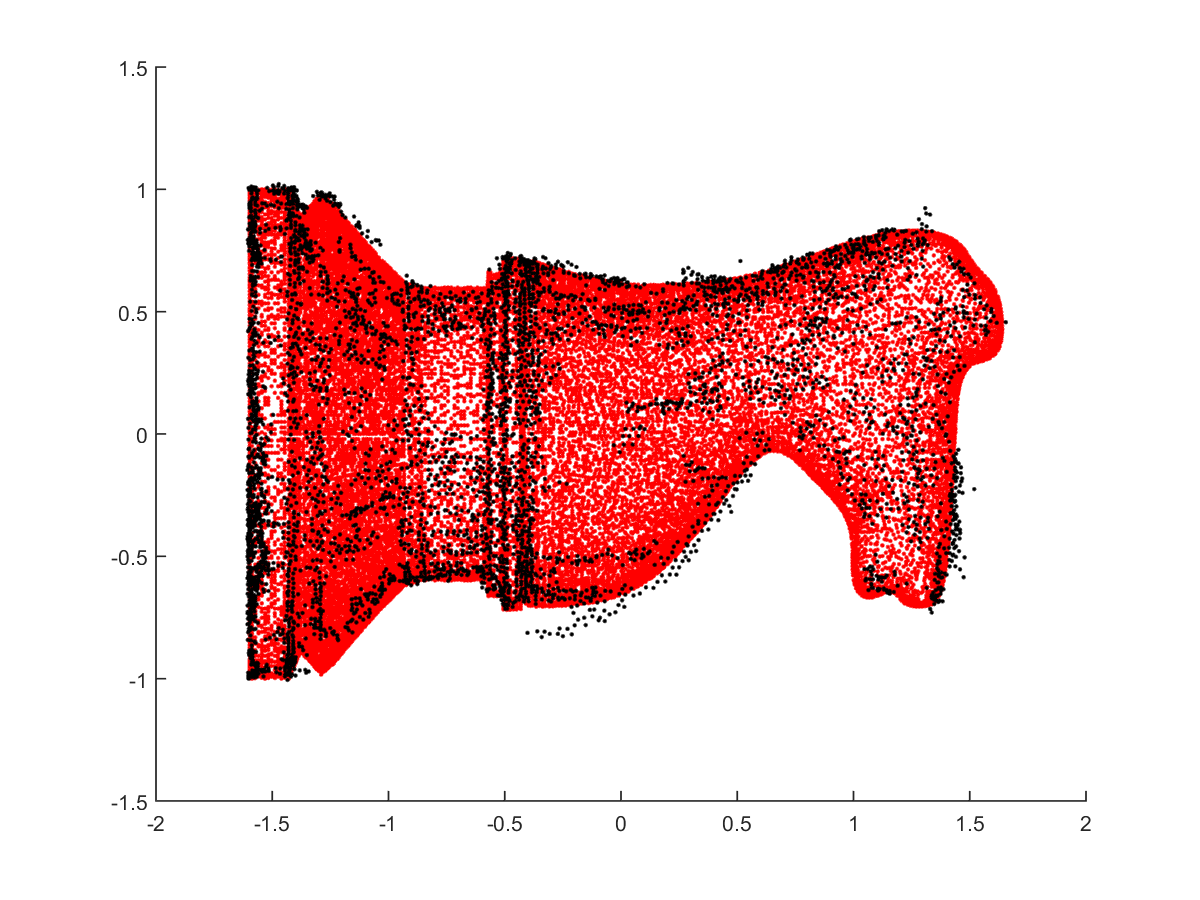
\includegraphics[width=0.2\textwidth]{interp/synth_data/knight/knight_mvs_02080502.png}&
  \fcolorbox{red}{white}{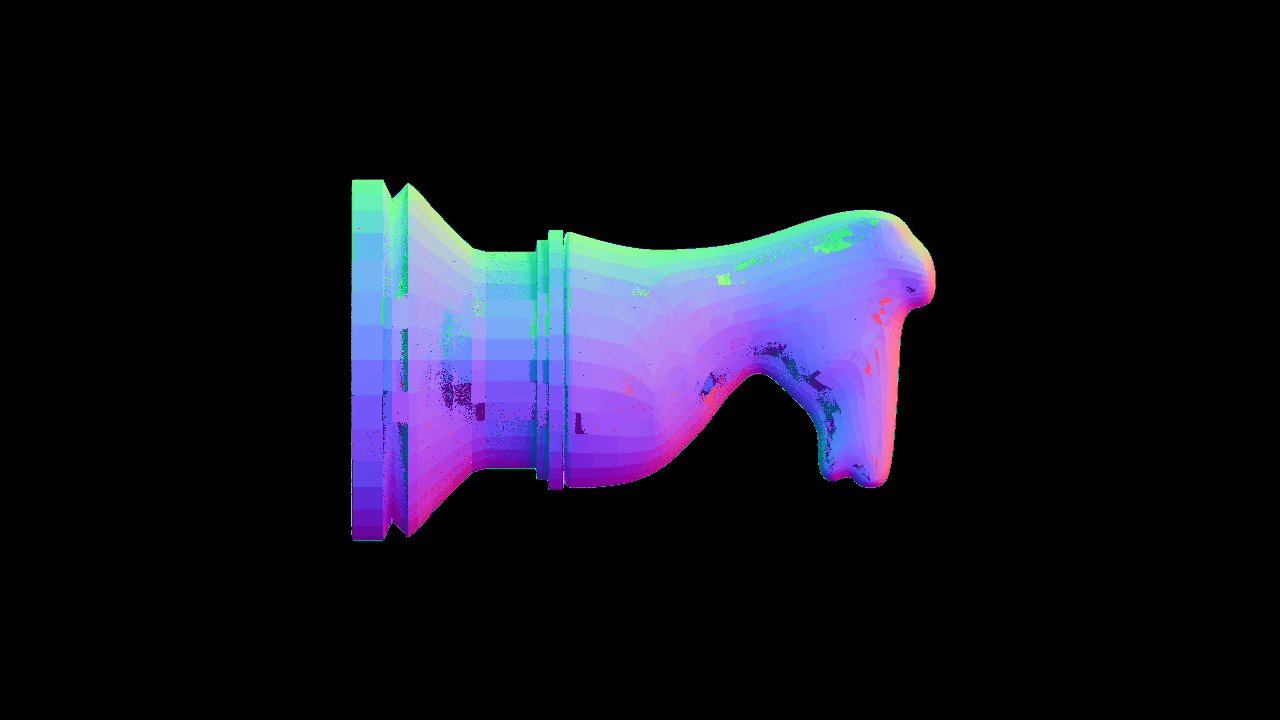
\includegraphics[width=0.2\textwidth]{interp/synth_data/knight/knight_ps_02080502.png}}&
  \fcolorbox{red}{white}{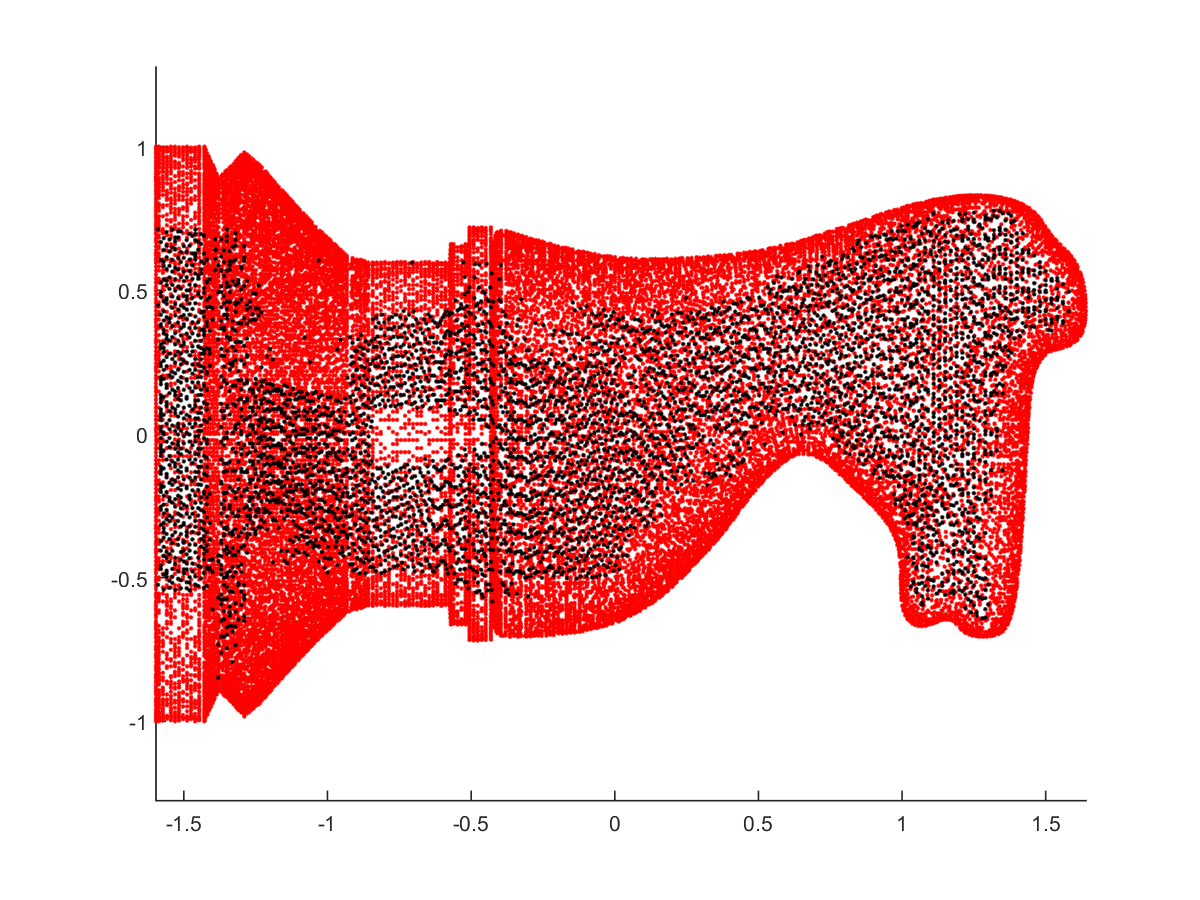
\includegraphics[width=0.2\textwidth]{interp/synth_data/knight/knight_sl_02080502.png}}\\
  & \multicolumn{4}{c}{(b). tex(0.2), alb(0.8), spec(0.5), rough(0.2)}\\
  MVS, PS, SL&
  \includegraphics[width=0.2\textwidth]{interp/synth_data/knight/knight_08080208}&
  \fcolorbox{red}{white}{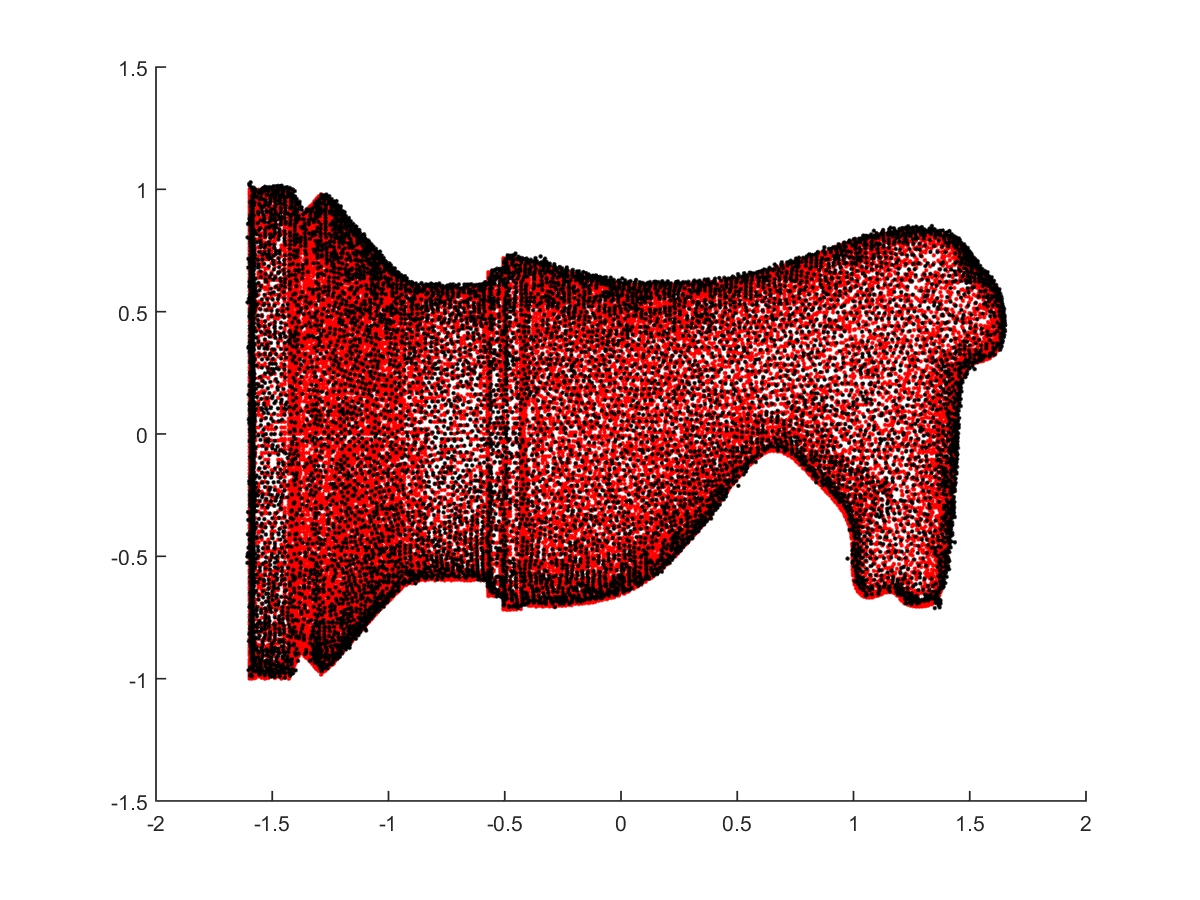
\includegraphics[width=0.2\textwidth]{interp/synth_data/knight/knight_mvs_08080208.png}}&
  \fcolorbox{red}{white}{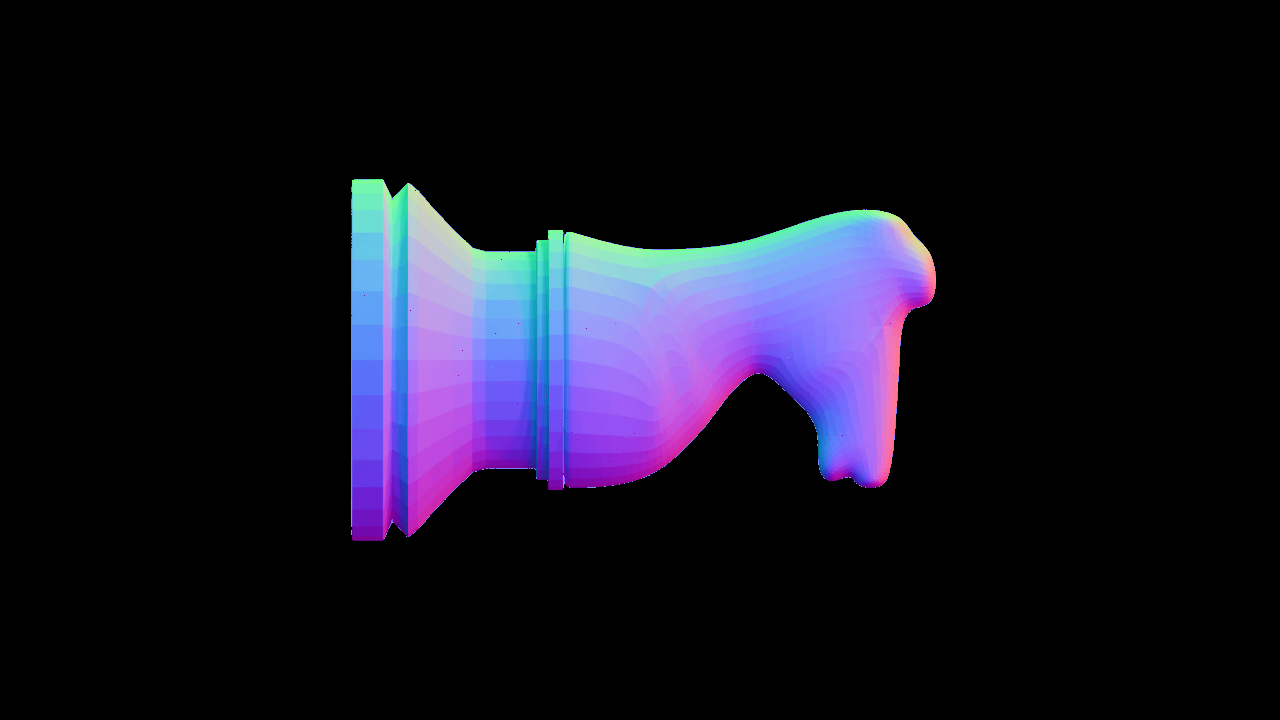
\includegraphics[width=0.2\textwidth]{interp/synth_data/knight/knight_ps_08080208.png}}&
  \fcolorbox{red}{white}{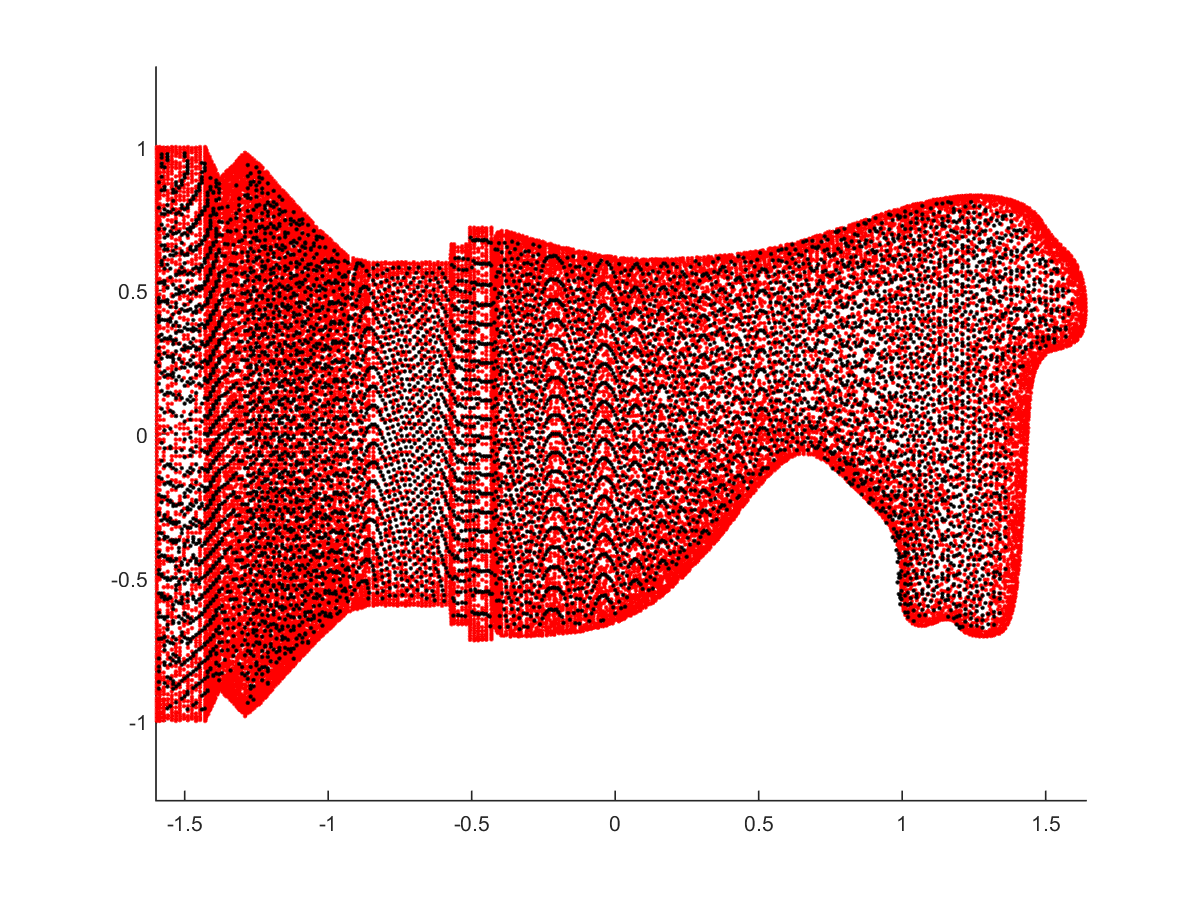
\includegraphics[width=0.2\textwidth]{interp/synth_data/knight/knight_sl_08080208.png}}\\
  & \multicolumn{4}{c}{(c). tex(0.8), alb(0.8), spec(0.2), rough(0.8)}\\
  MVS, PS, SL&
  \includegraphics[width=0.2\textwidth]{interp/synth_data/knight/knight_08080502}&
  \fcolorbox{red}{white}{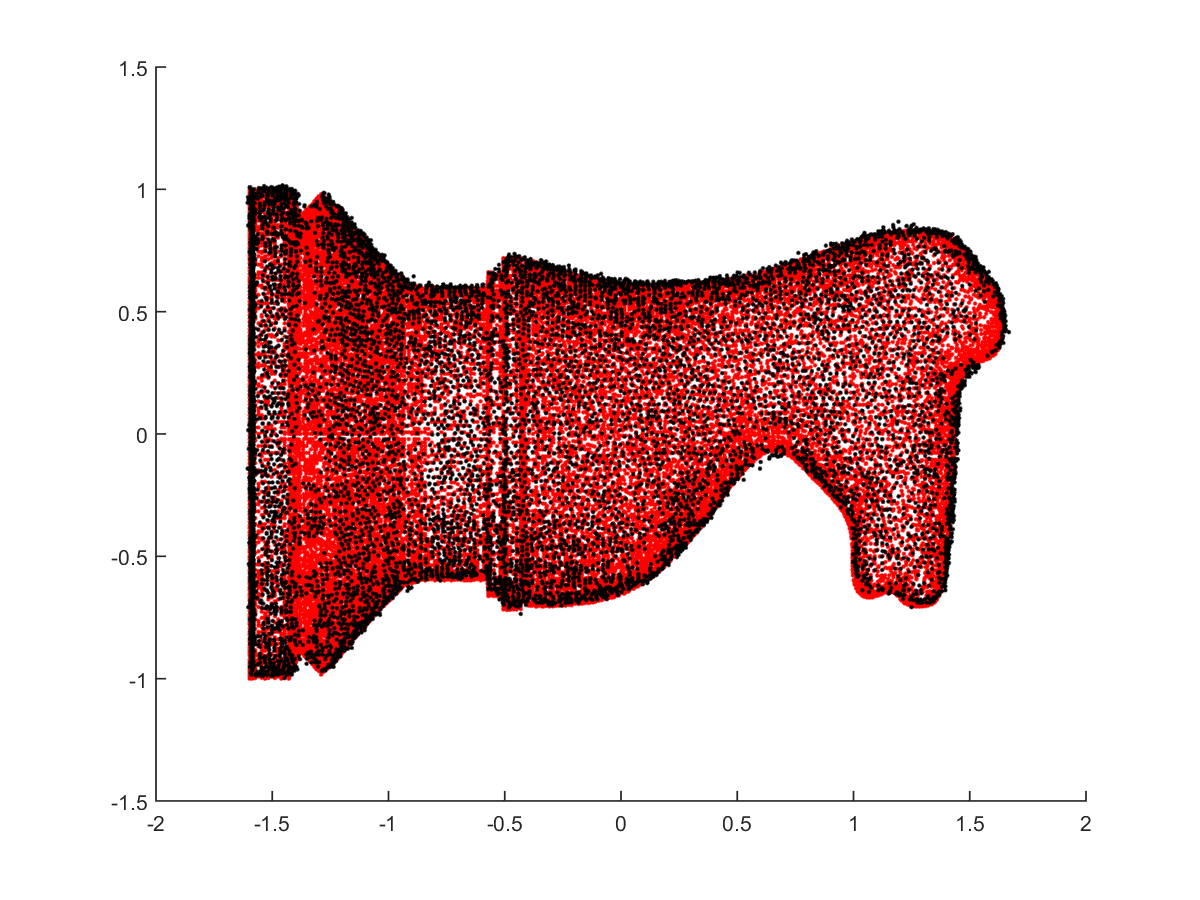
\includegraphics[width=0.2\textwidth]{interp/synth_data/knight/knight_mvs_08080502.png}}&
  \fcolorbox{red}{white}{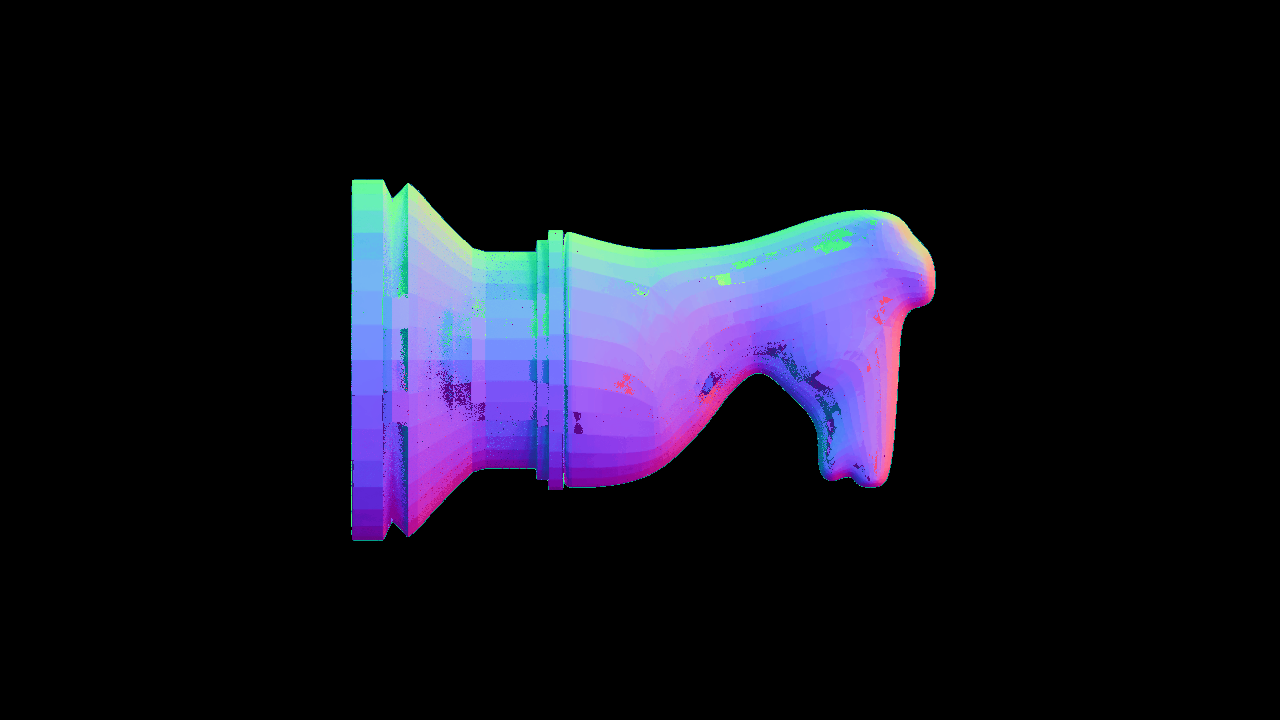
\includegraphics[width=0.2\textwidth]{interp/synth_data/knight/knight_ps_08080502.png}}&
  \fcolorbox{red}{white}{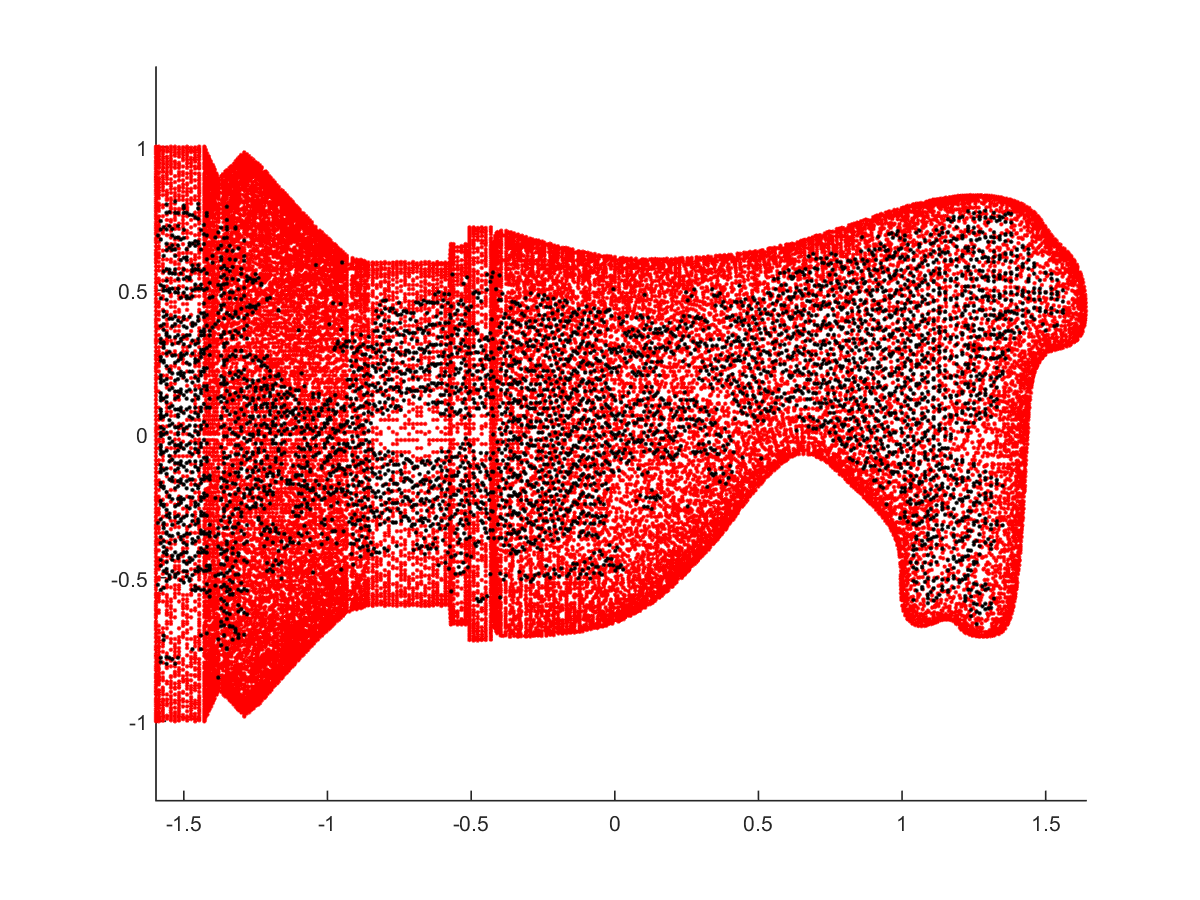
\includegraphics[width=0.2\textwidth]{interp/synth_data/knight/knight_sl_08080502.png}}\\
  & \multicolumn{4}{c}{(d). tex(0.8), alb(0.8), spec(0.5), rough(0.2)}\\
  \hline
  ~ & ~ & MVS & PS & SL\\
\end{tabular}
\caption{The first column shows the best algorithm chosen by the mapping. The quantitative and qualitative performance of each technique on the synthetic dataset. The red dots are from the ground truth while the black ones the reconstruction.}
\label{fig:synth_data_results}
\end{sidewaysfigure}

\subsubsection{Results}
\textbf{(a), (b)} In Figure~\ref{fig:synth_data_results} (a), the mapping predicts that EPS and GSL can give satisfactory results, which is consistent to the quantitative result shown in column 2 and the qualitative resulted labeled in red rectangle. The completeness of the PMVS is low due to the lack of texture.

\textbf{(c), (d)} In Figure~\ref{fig:synth_data_results} (a), the mapping predicts that all three methods can give satisfactory results, which is consistent to the quantitative result shown in column 2 and the qualitative resulted labeled in red rectangle.

\subsection{Real-world Datasets}
We used a similar setup to the synthetic settings and captured a real world dataset for nine objects. The property of these objects are listed in Table~\ref{tab:prop_list_real_data}. Since we don't have the ground truth, we resort to visual analysis to see if the algorithm gives the best reconstruction is consistent to the algorithm suggested by the mapping. We choose four representative objects as representatives of the six classes of objects, they are
\begin{figure}[!htbp]
\centering
\begin{tabular}{c|cccc}
\hline
class \# & 1 & 2 & 3\&4 & 5\&6\\
\hline
  & textureless & textureless & textured & textured\\
description & diffuse & mixed d/s & diffuse & mixed d/s\\
  & bright & bright & dark/bright & dark/bright\\
\hline
object & 
\raisebox{-.5\height}{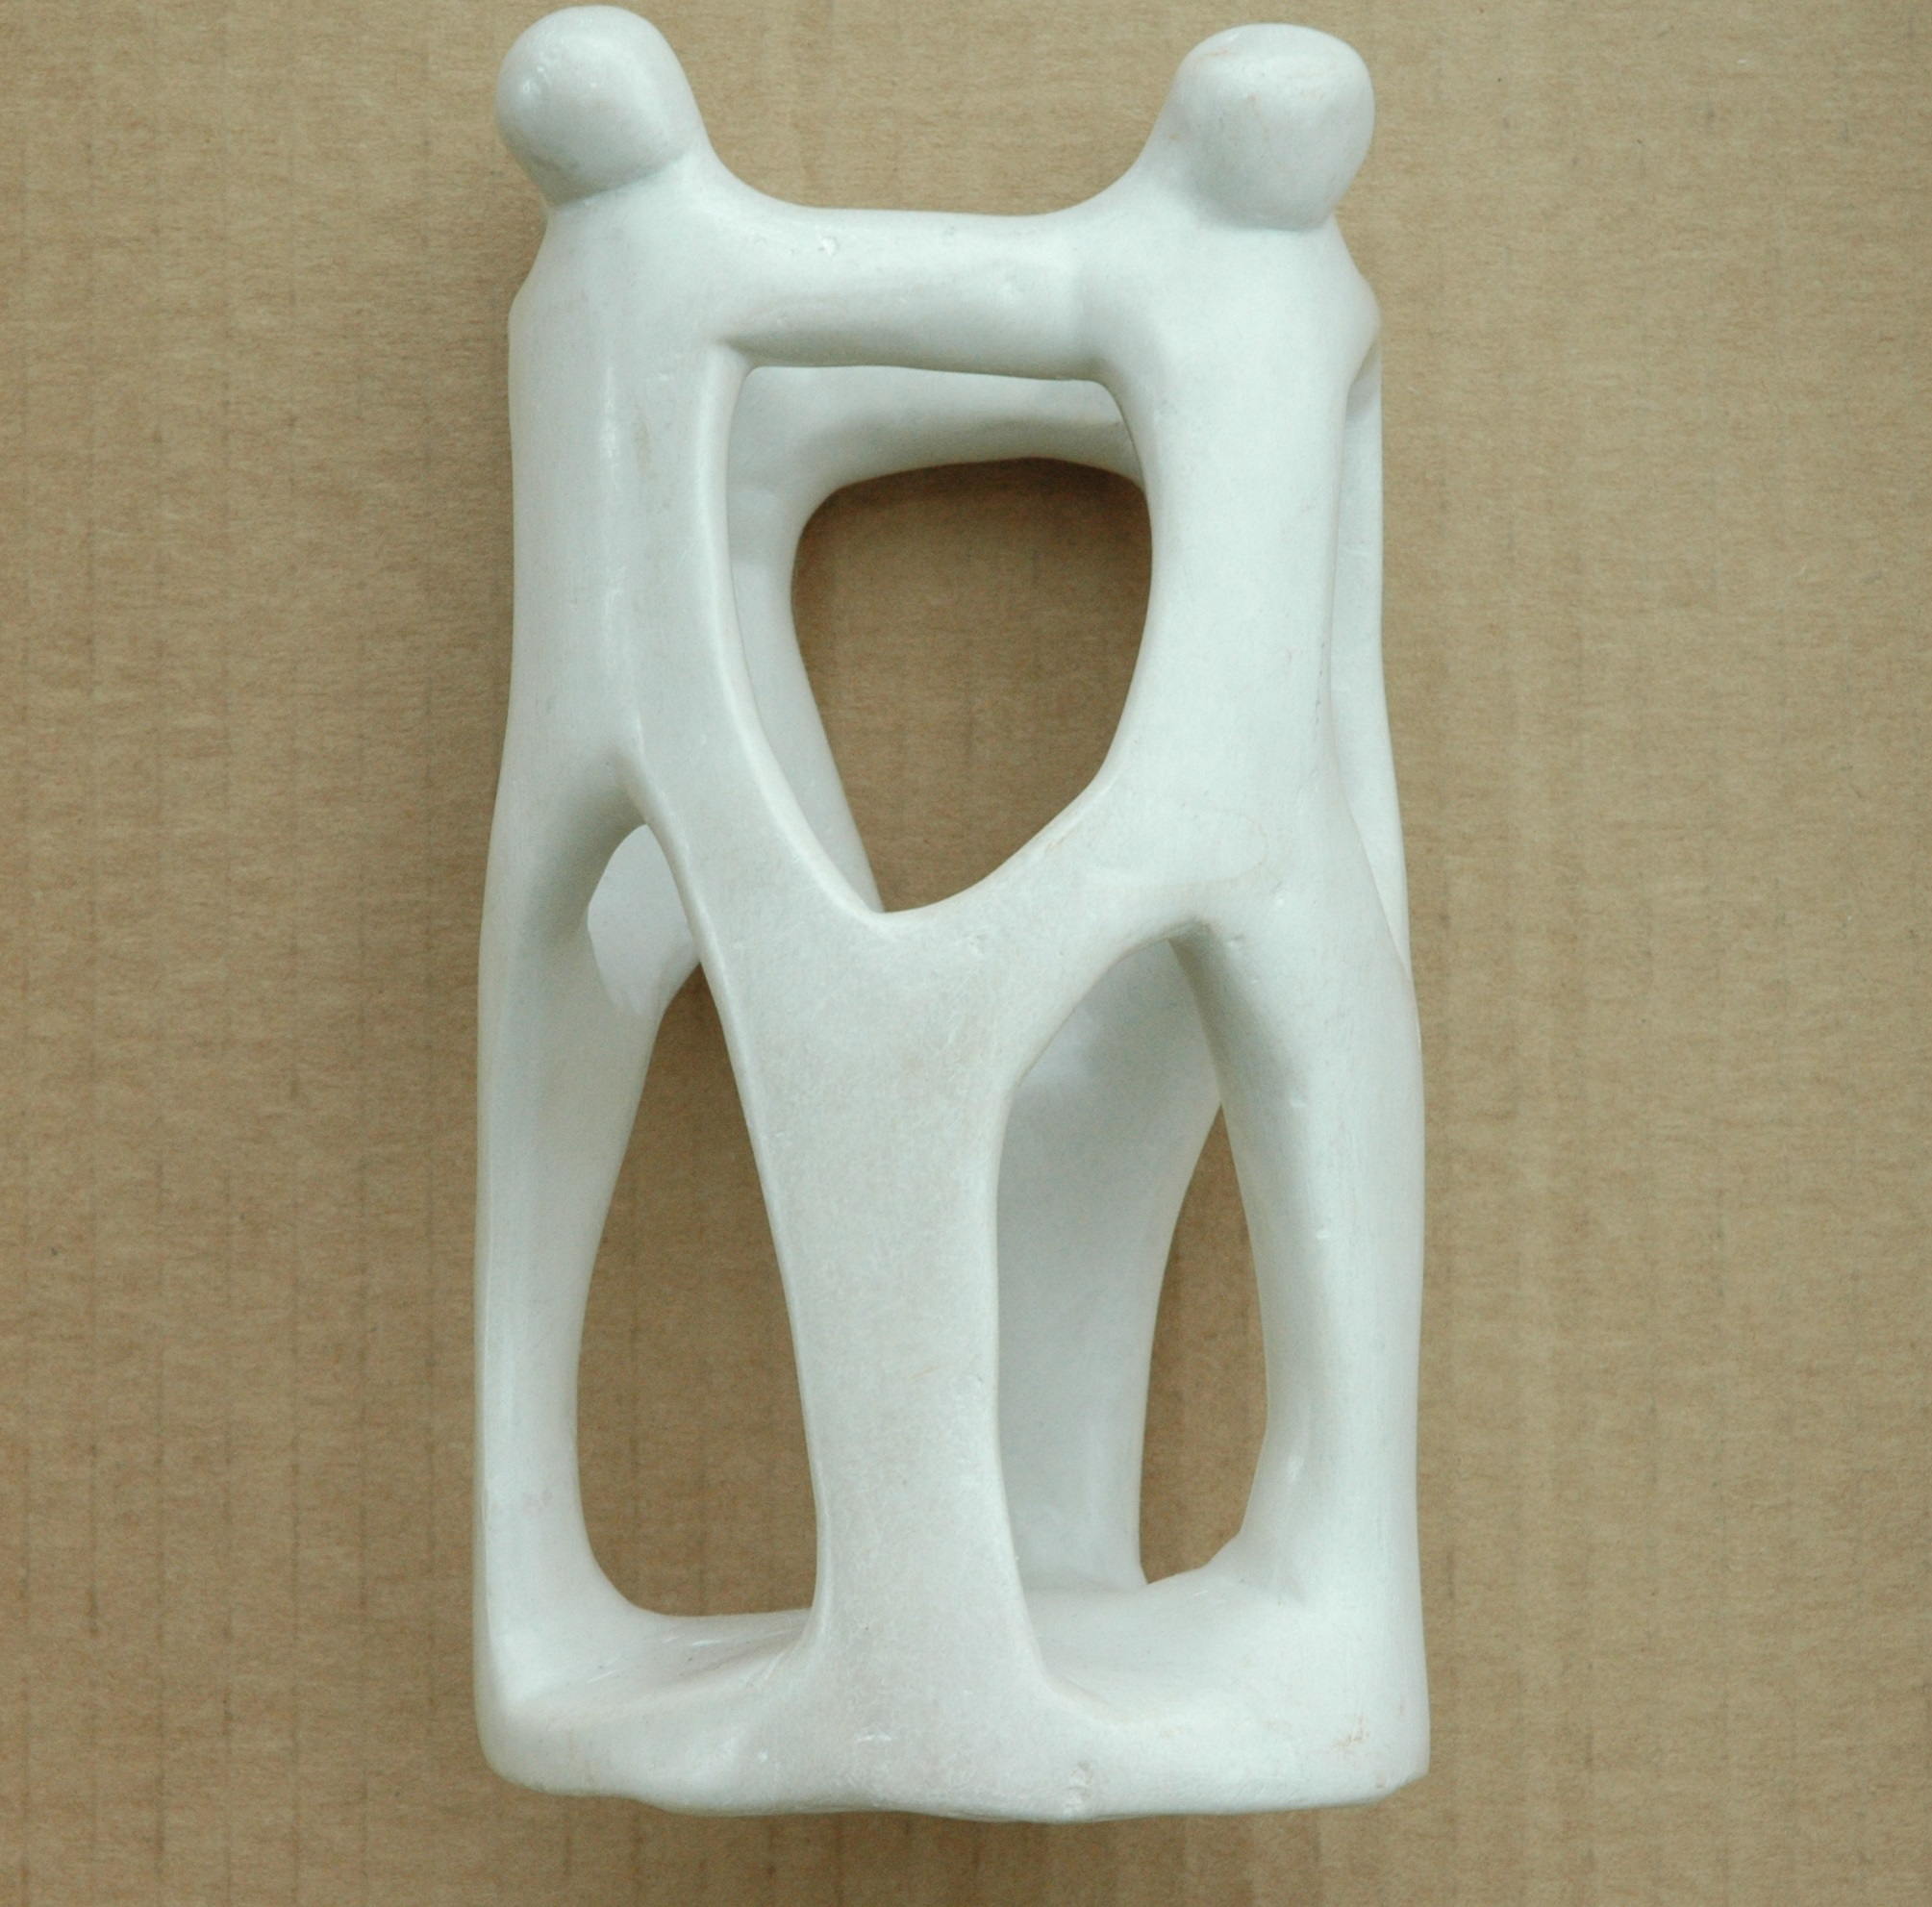
\includegraphics[width=0.22\textwidth]{interp/real_world_obj/statue/statue}} &
\raisebox{-.5\height}{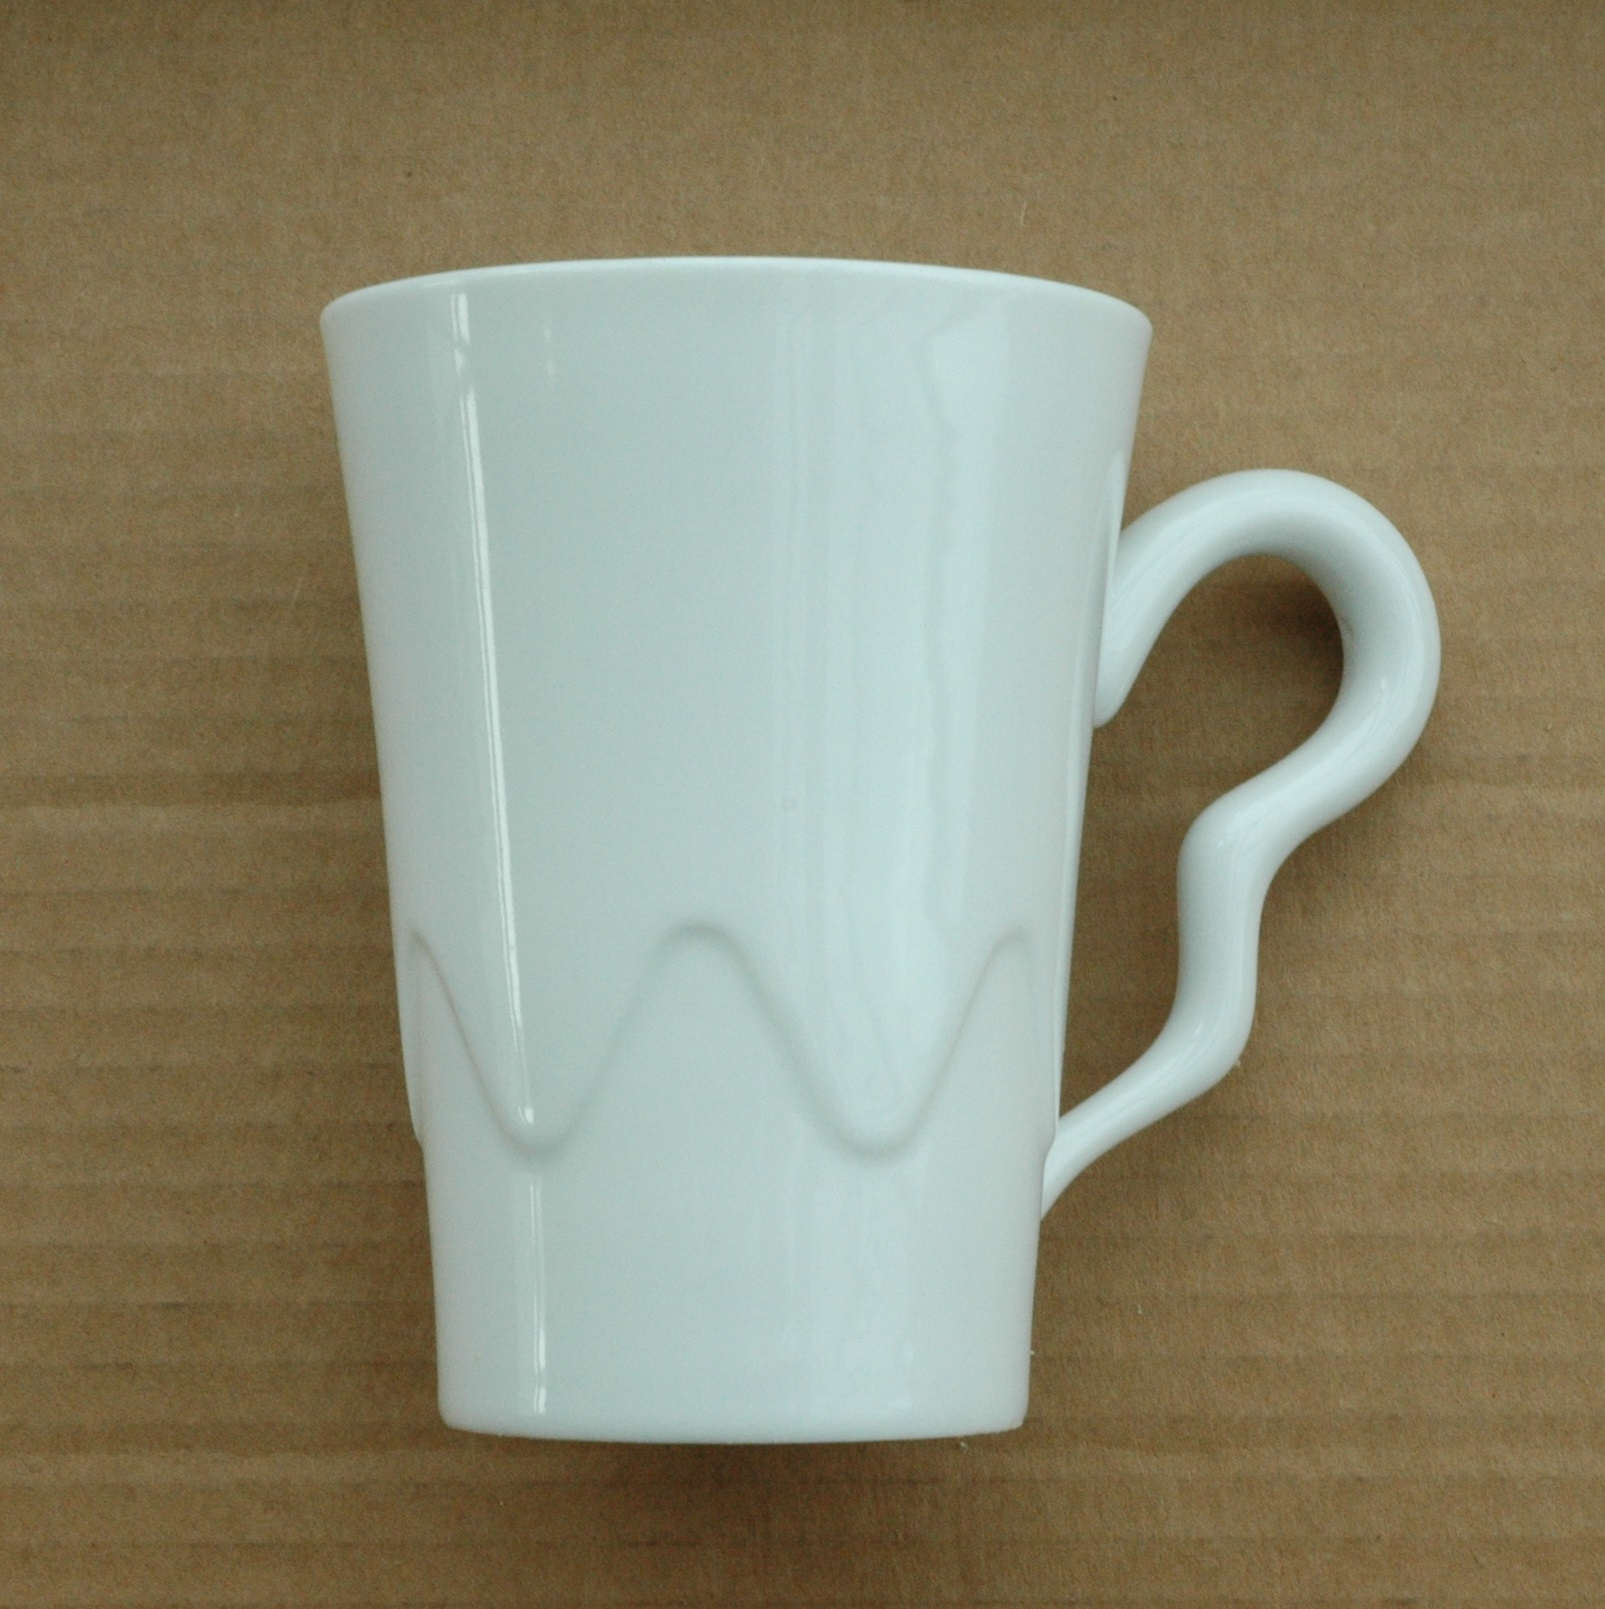
\includegraphics[width=0.22\textwidth]{interp/real_world_obj/cup/cup}} &
\raisebox{-.5\height}{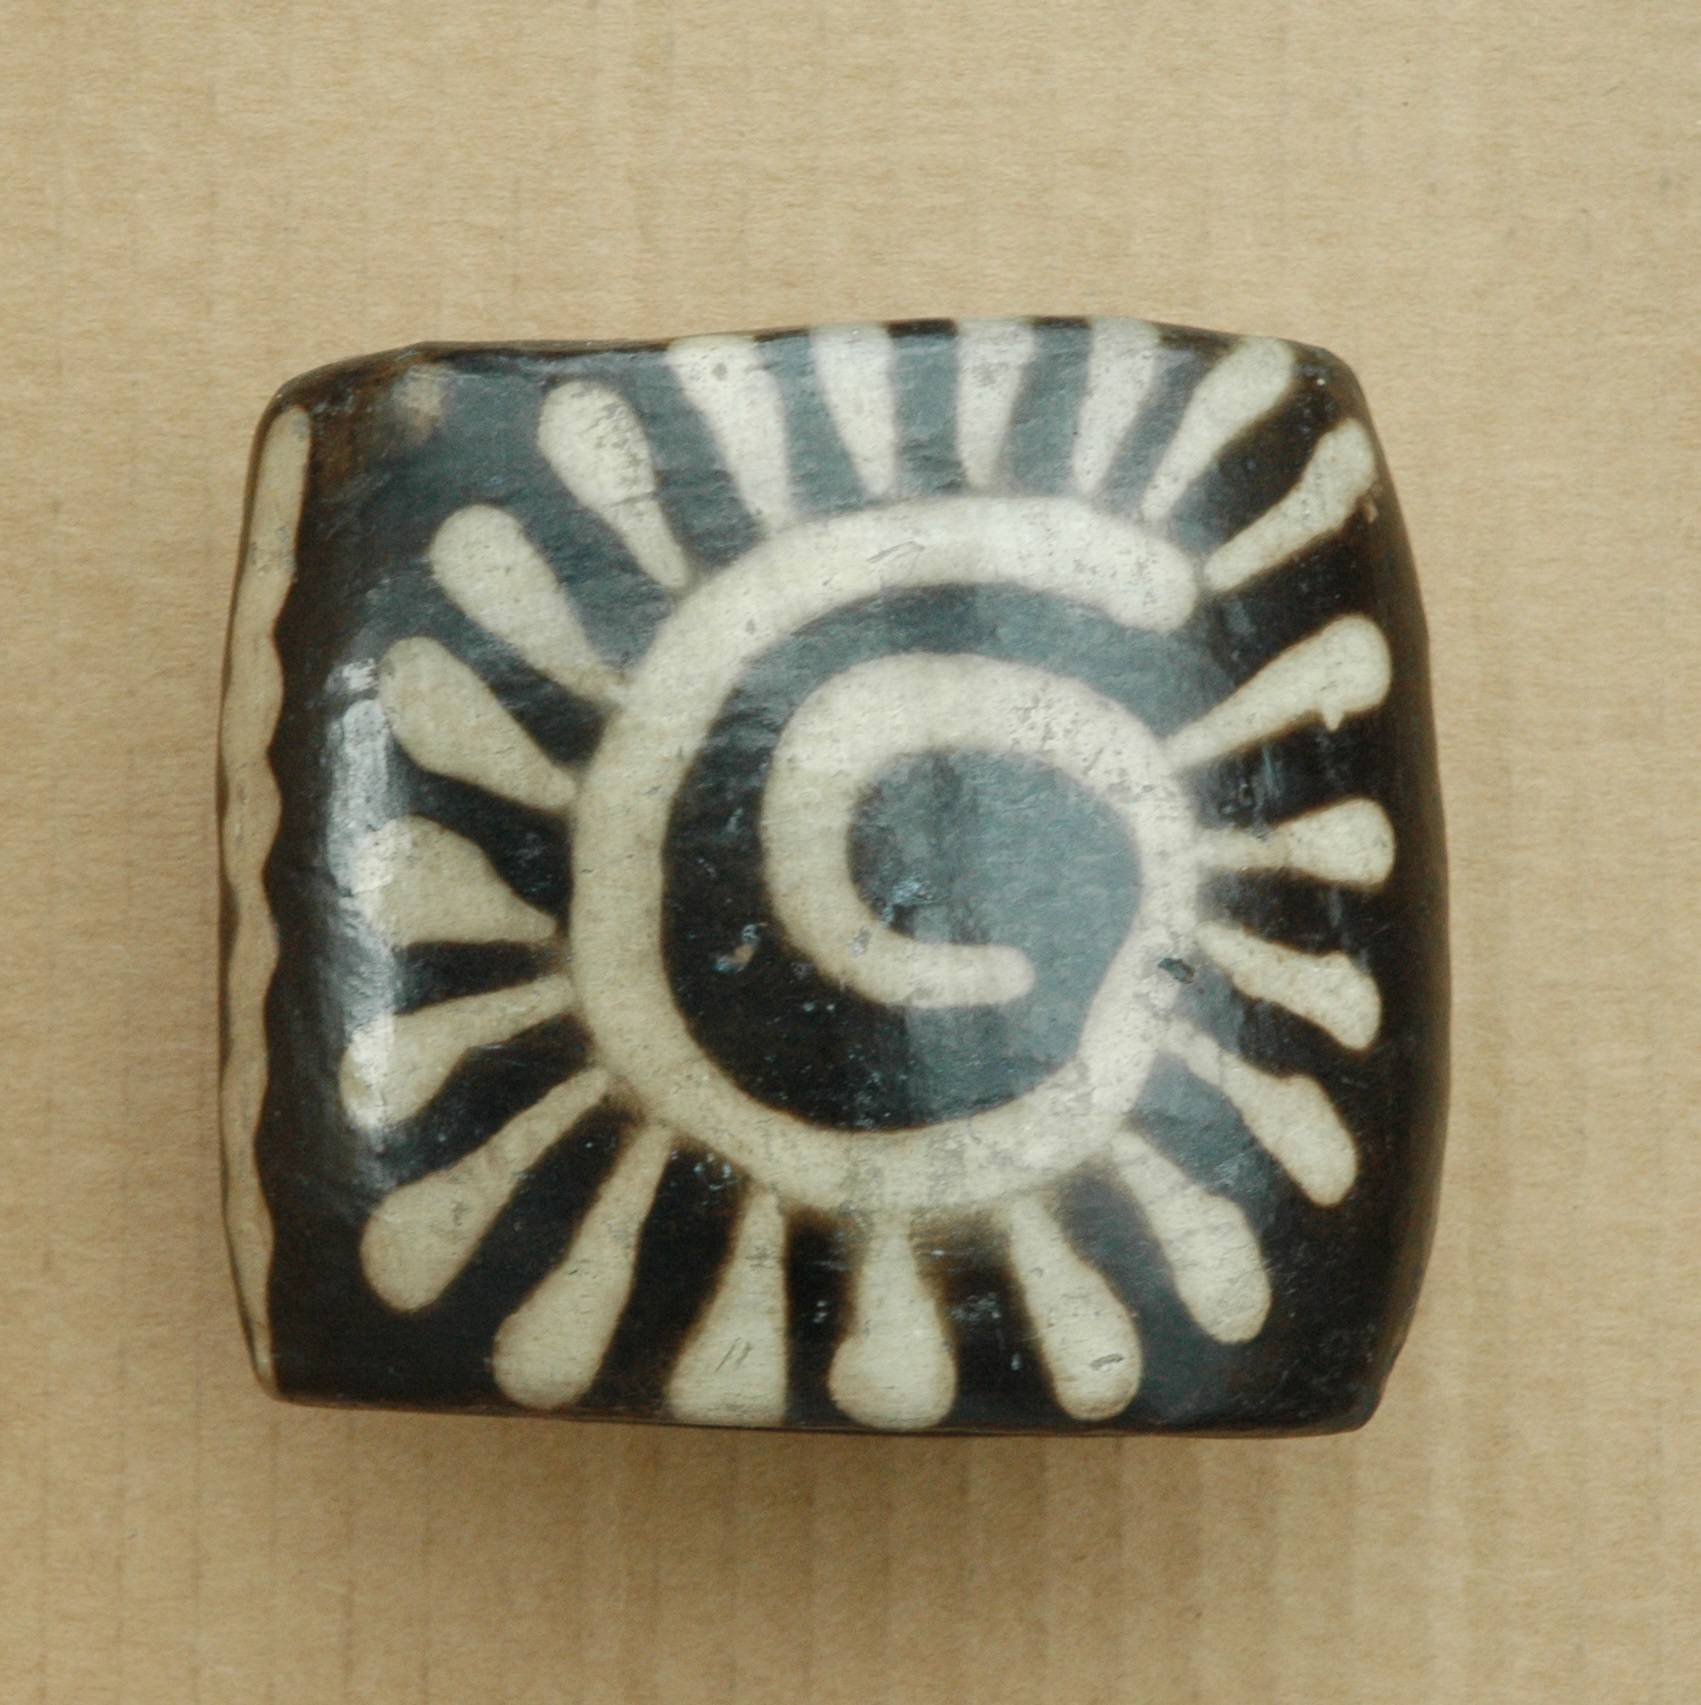
\includegraphics[width=0.22\textwidth]{interp/real_world_obj/pot/pot}} &
\raisebox{-.5\height}{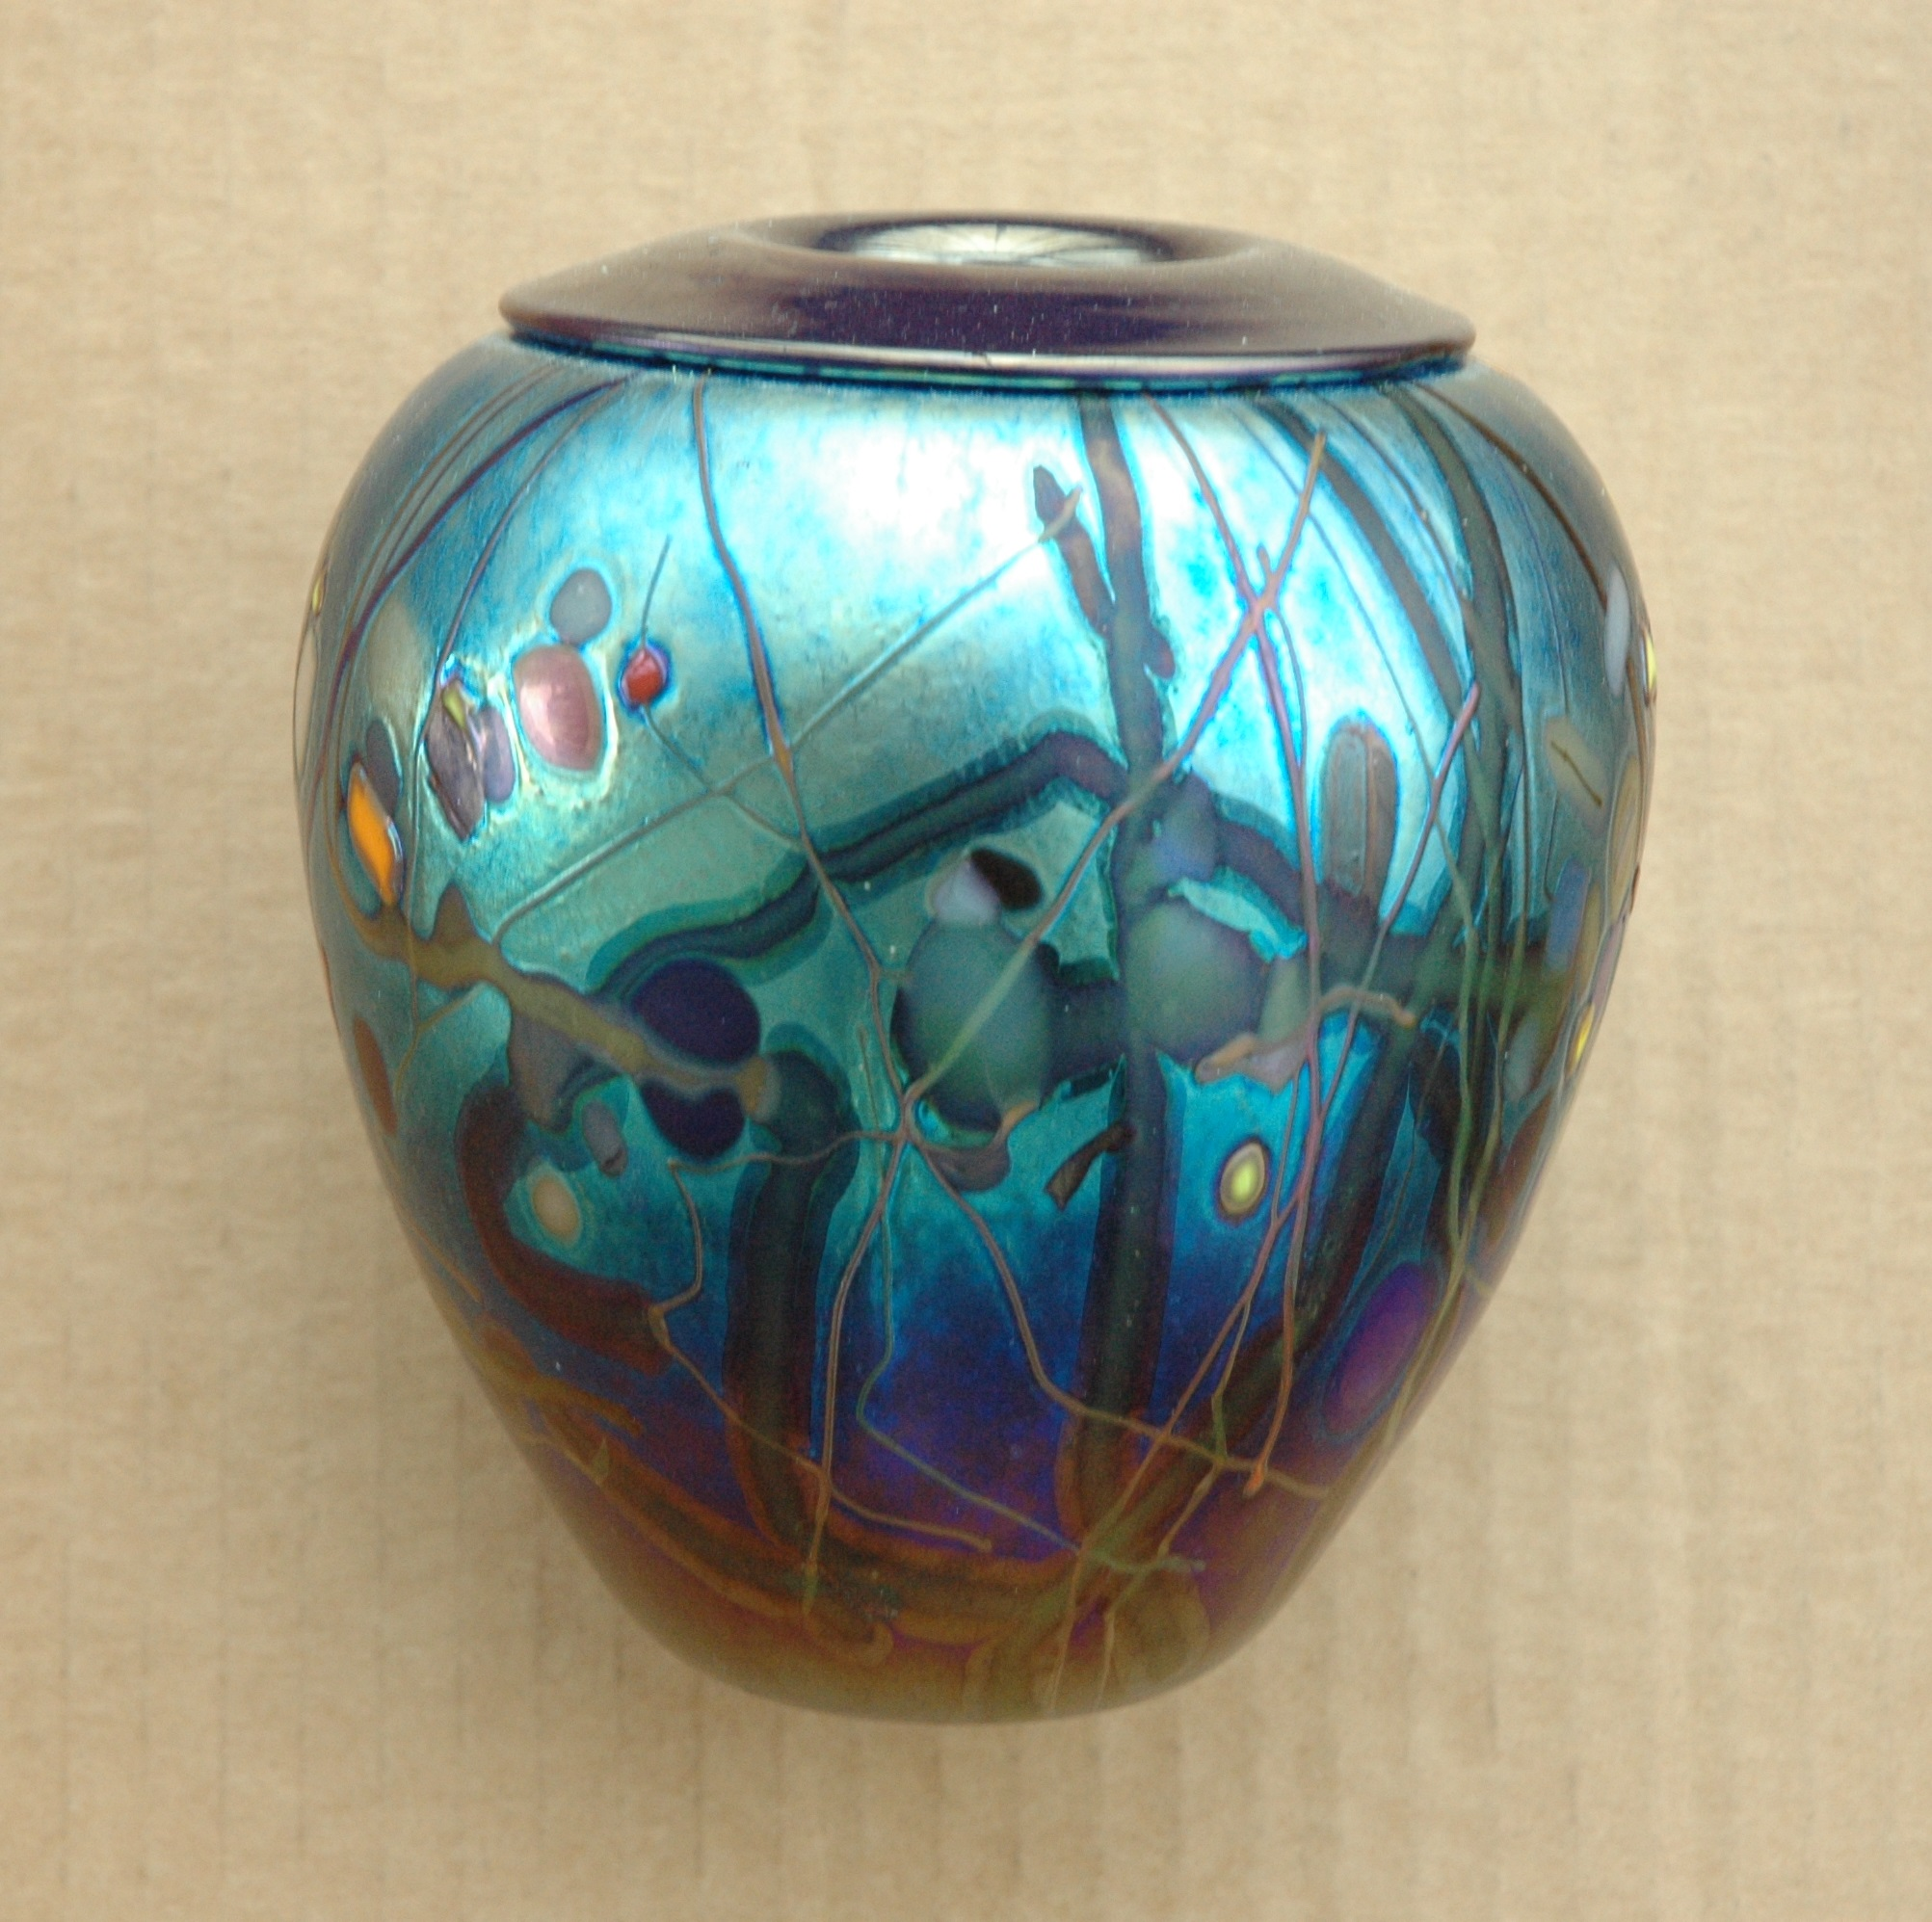
\includegraphics[width=0.22\textwidth]{interp/real_world_obj/vase/vase}}\\
\end{tabular}
\caption{The rerepsentatives of the six classes of objects used for evaluation.}
\label{fig:test_real_world_6class}
\end{figure}

We use the aforementioned methods to retrieve the parameters of each property, the decomposition of material for each object is presented in Figure~\ref{fig:real_data_material}.
% \begin{table}[!hbtp]
%   \centering
%   \begin{tabular}{*{12}{c}}
%   \multicolumn{3}{l}{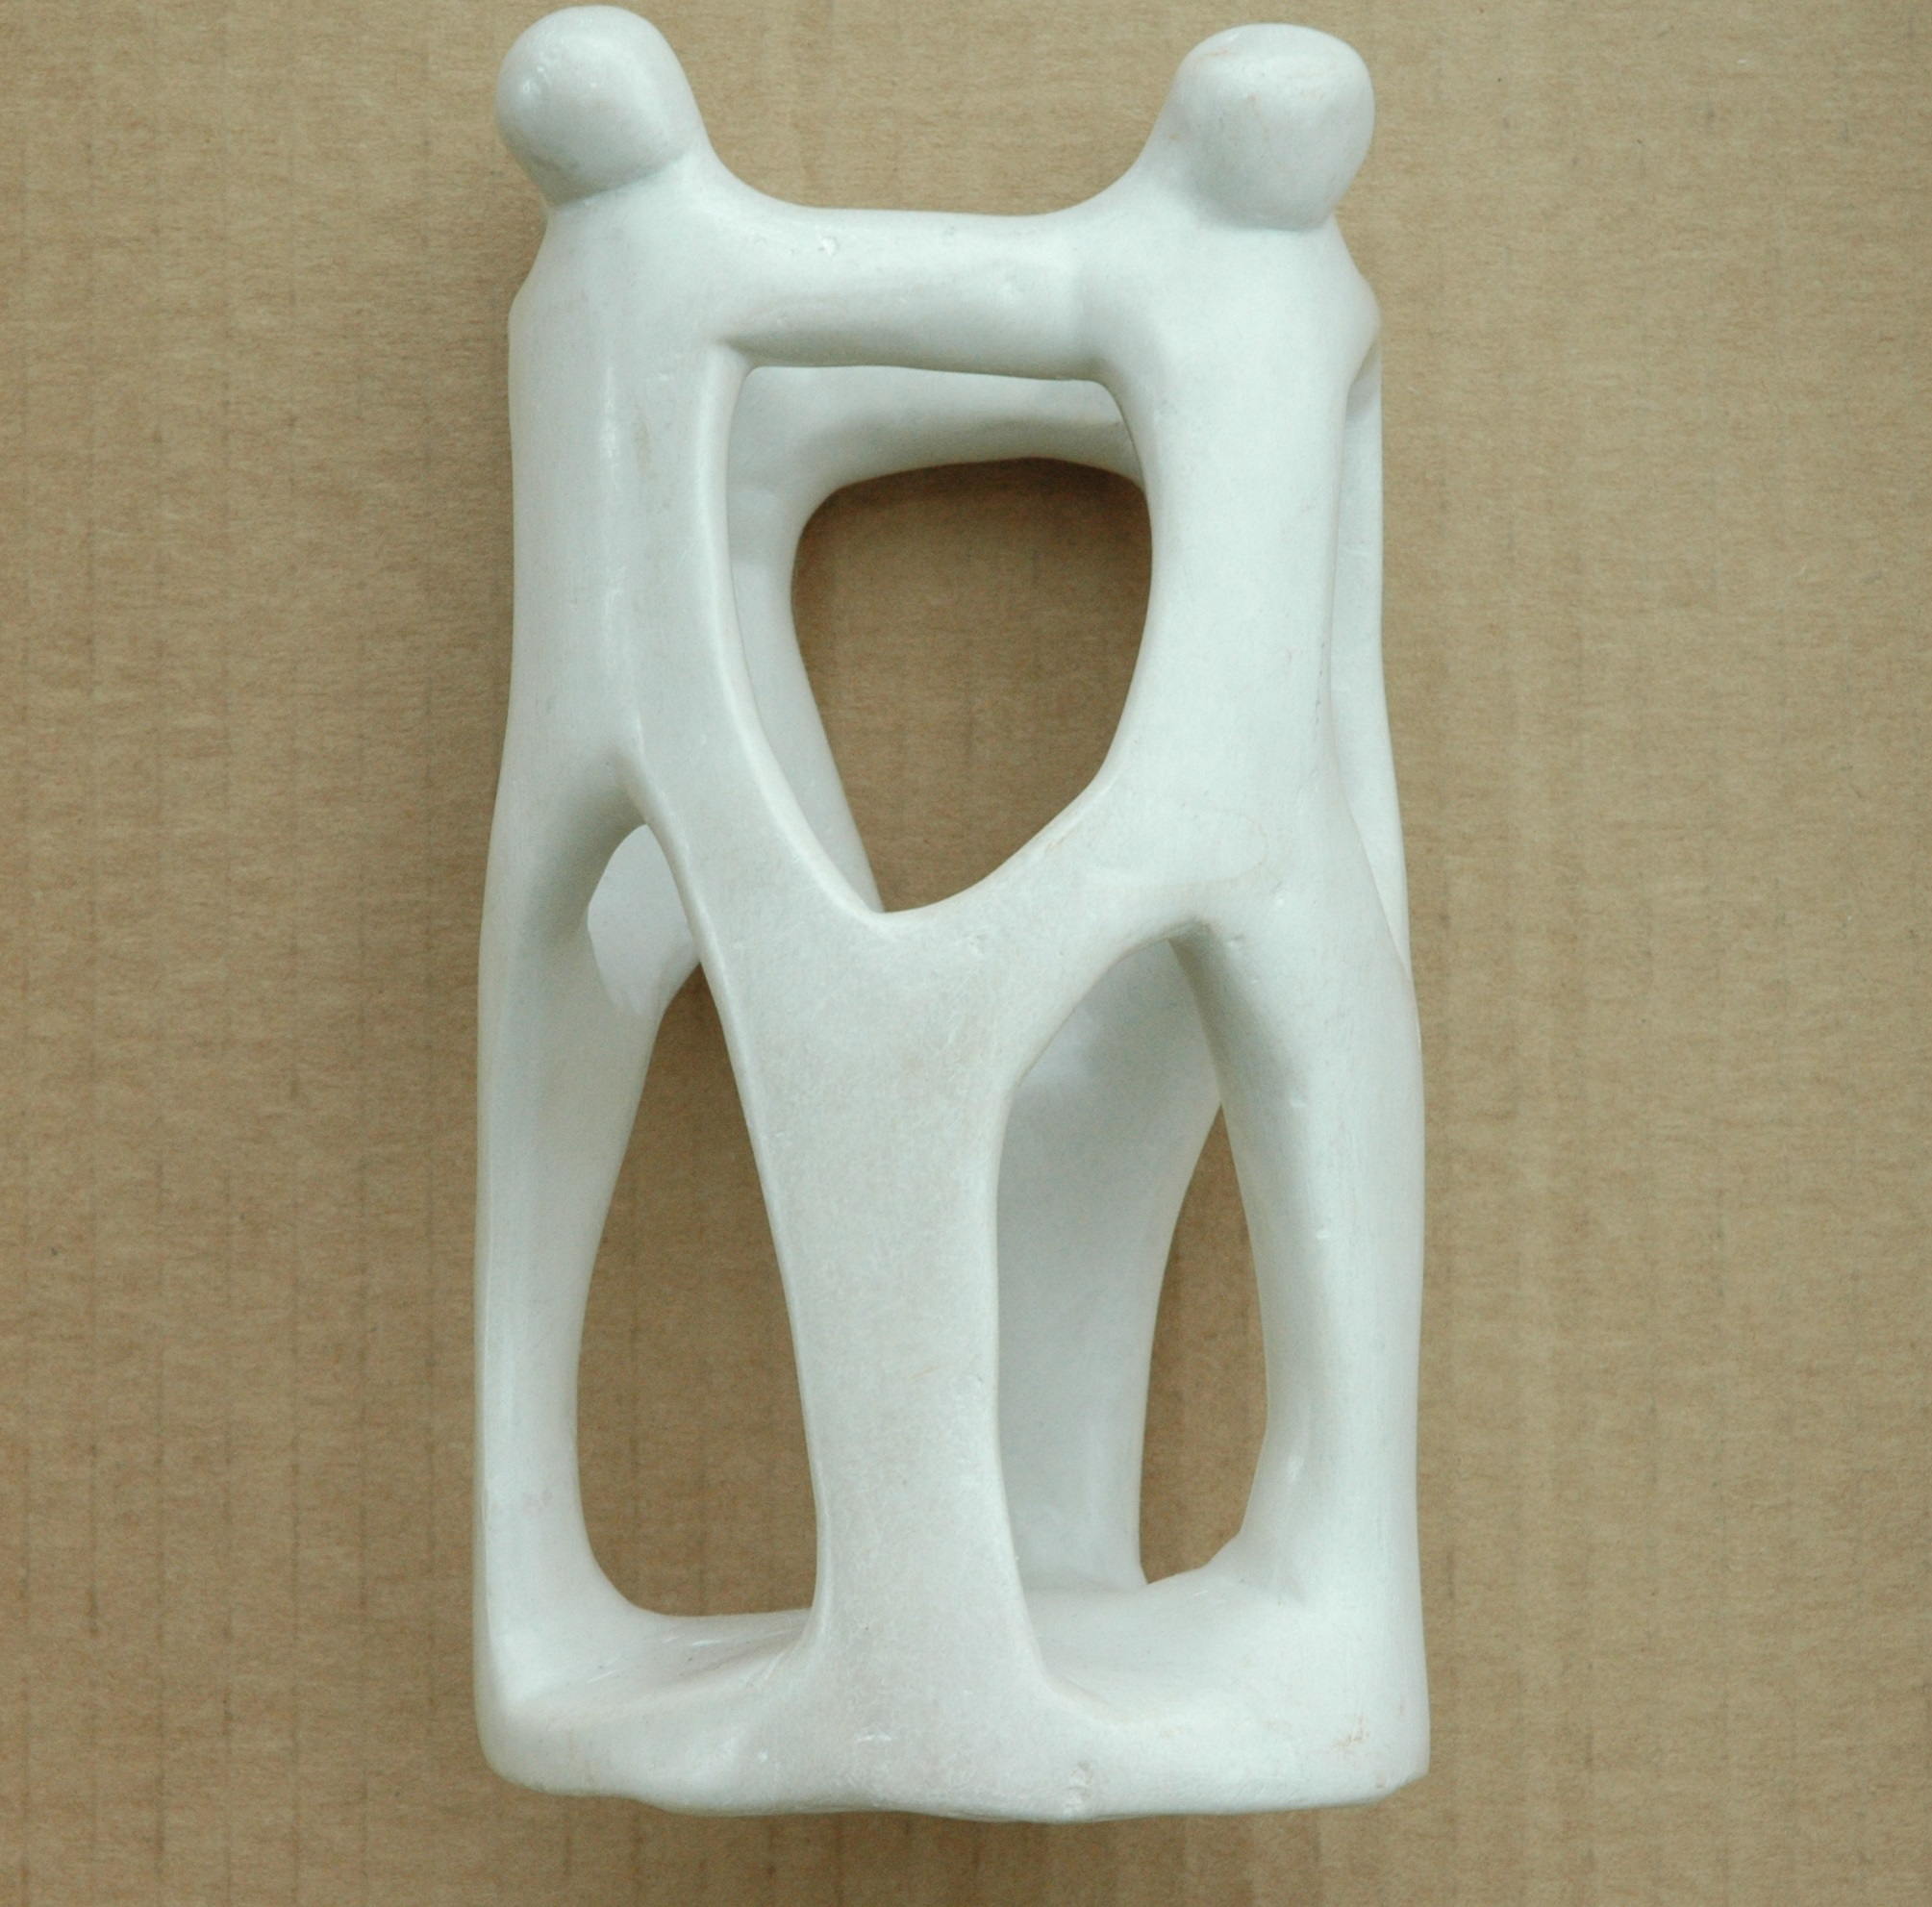
\includegraphics[width=0.25\textwidth]{interp/real_world_obj/statue/statue}} &
%   \multicolumn{3}{l}{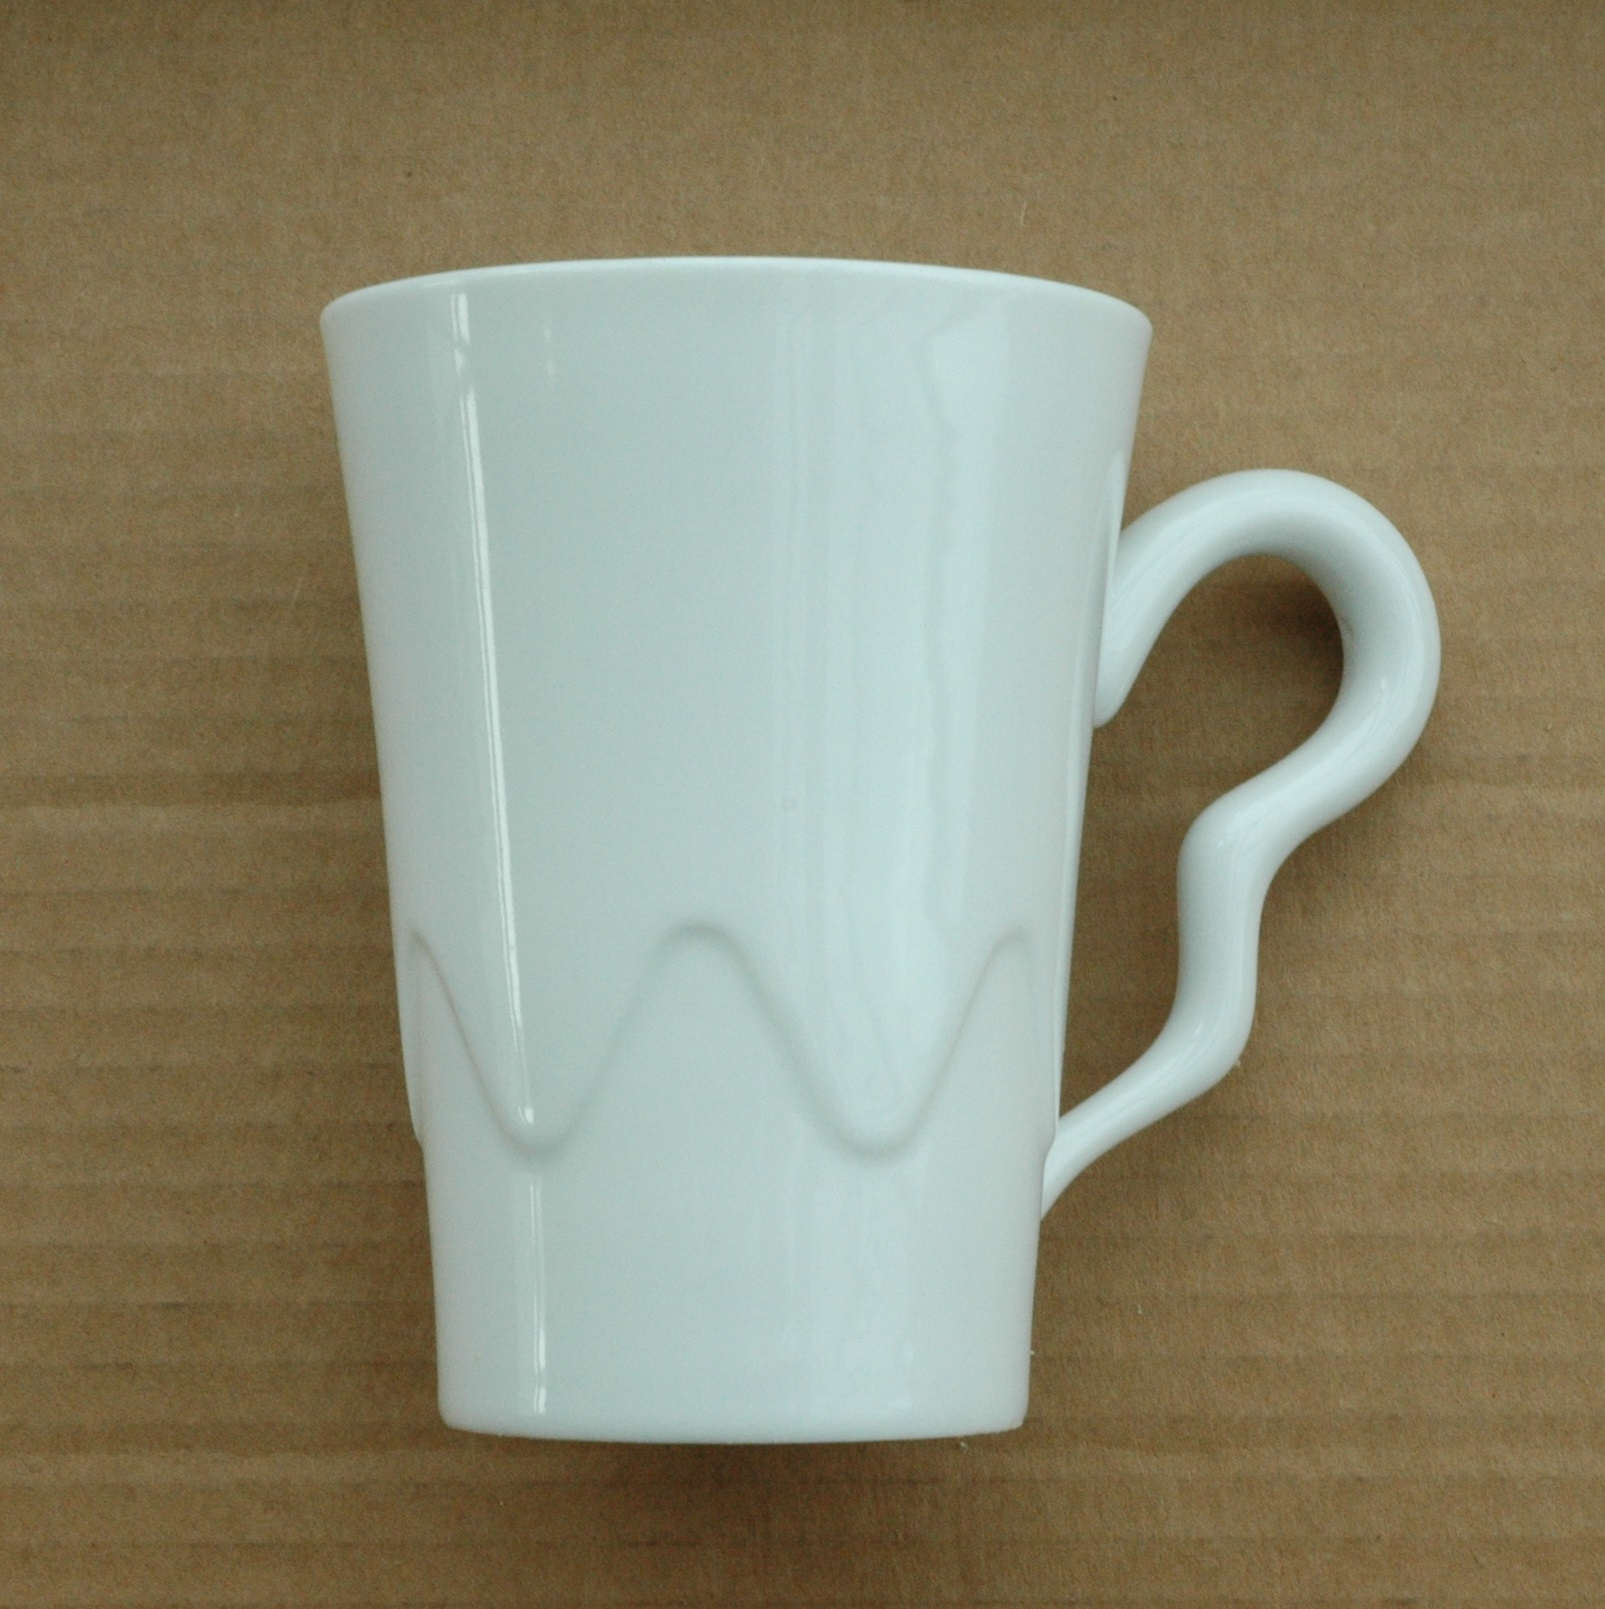
\includegraphics[width=0.25\textwidth]{interp/real_world_obj/cup/cup}} &
%   \multicolumn{3}{l}{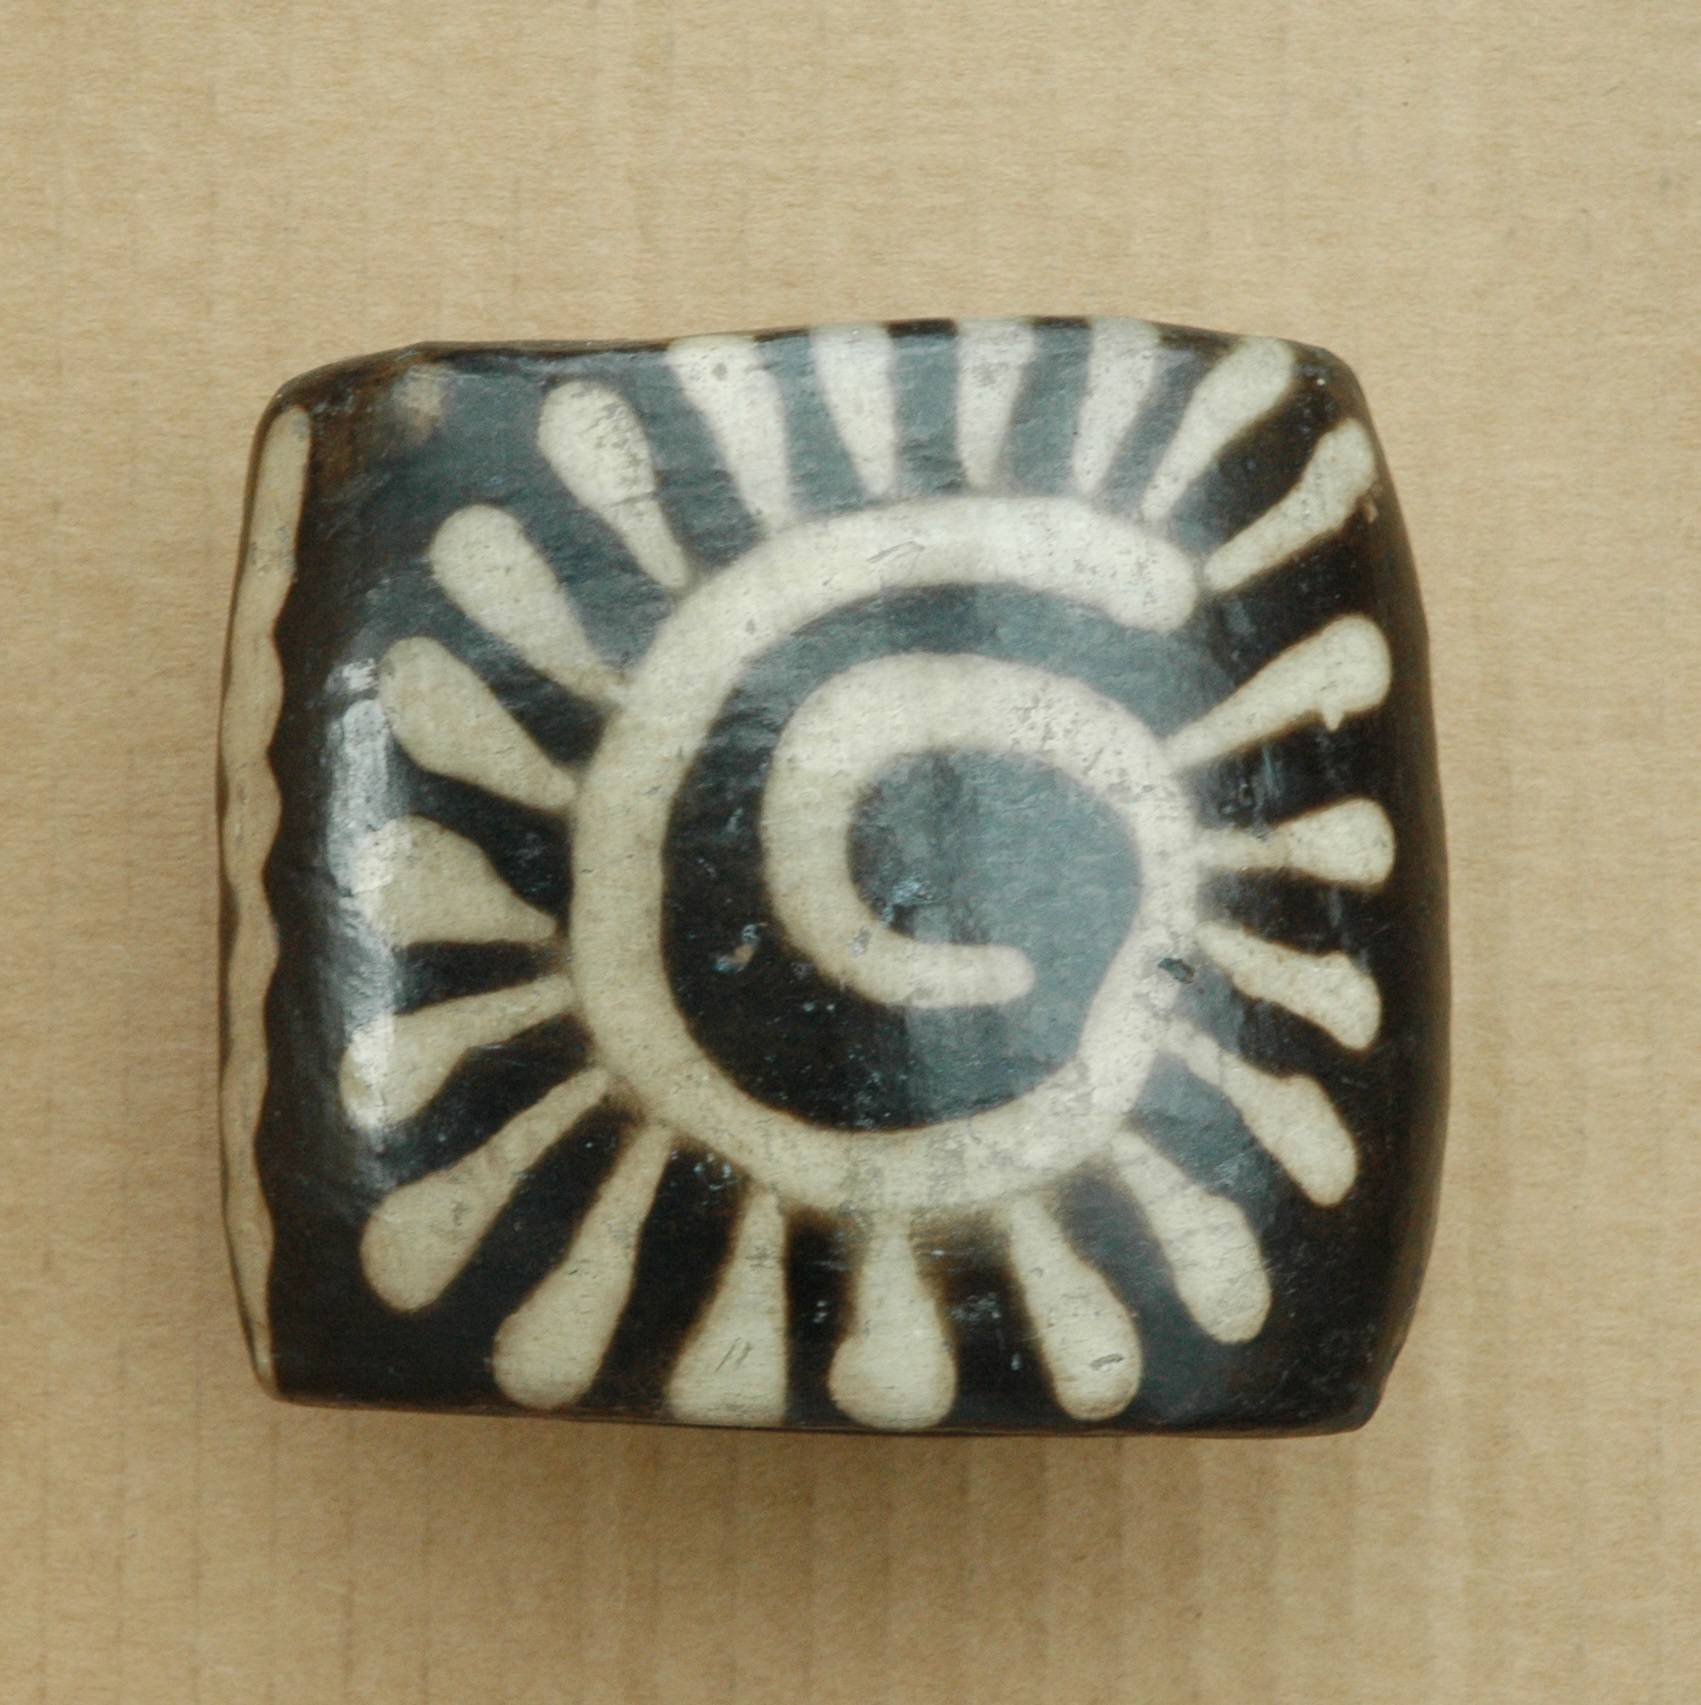
\includegraphics[width=0.25\textwidth]{interp/real_world_obj/pot/pot}} &
%   \multicolumn{3}{l}{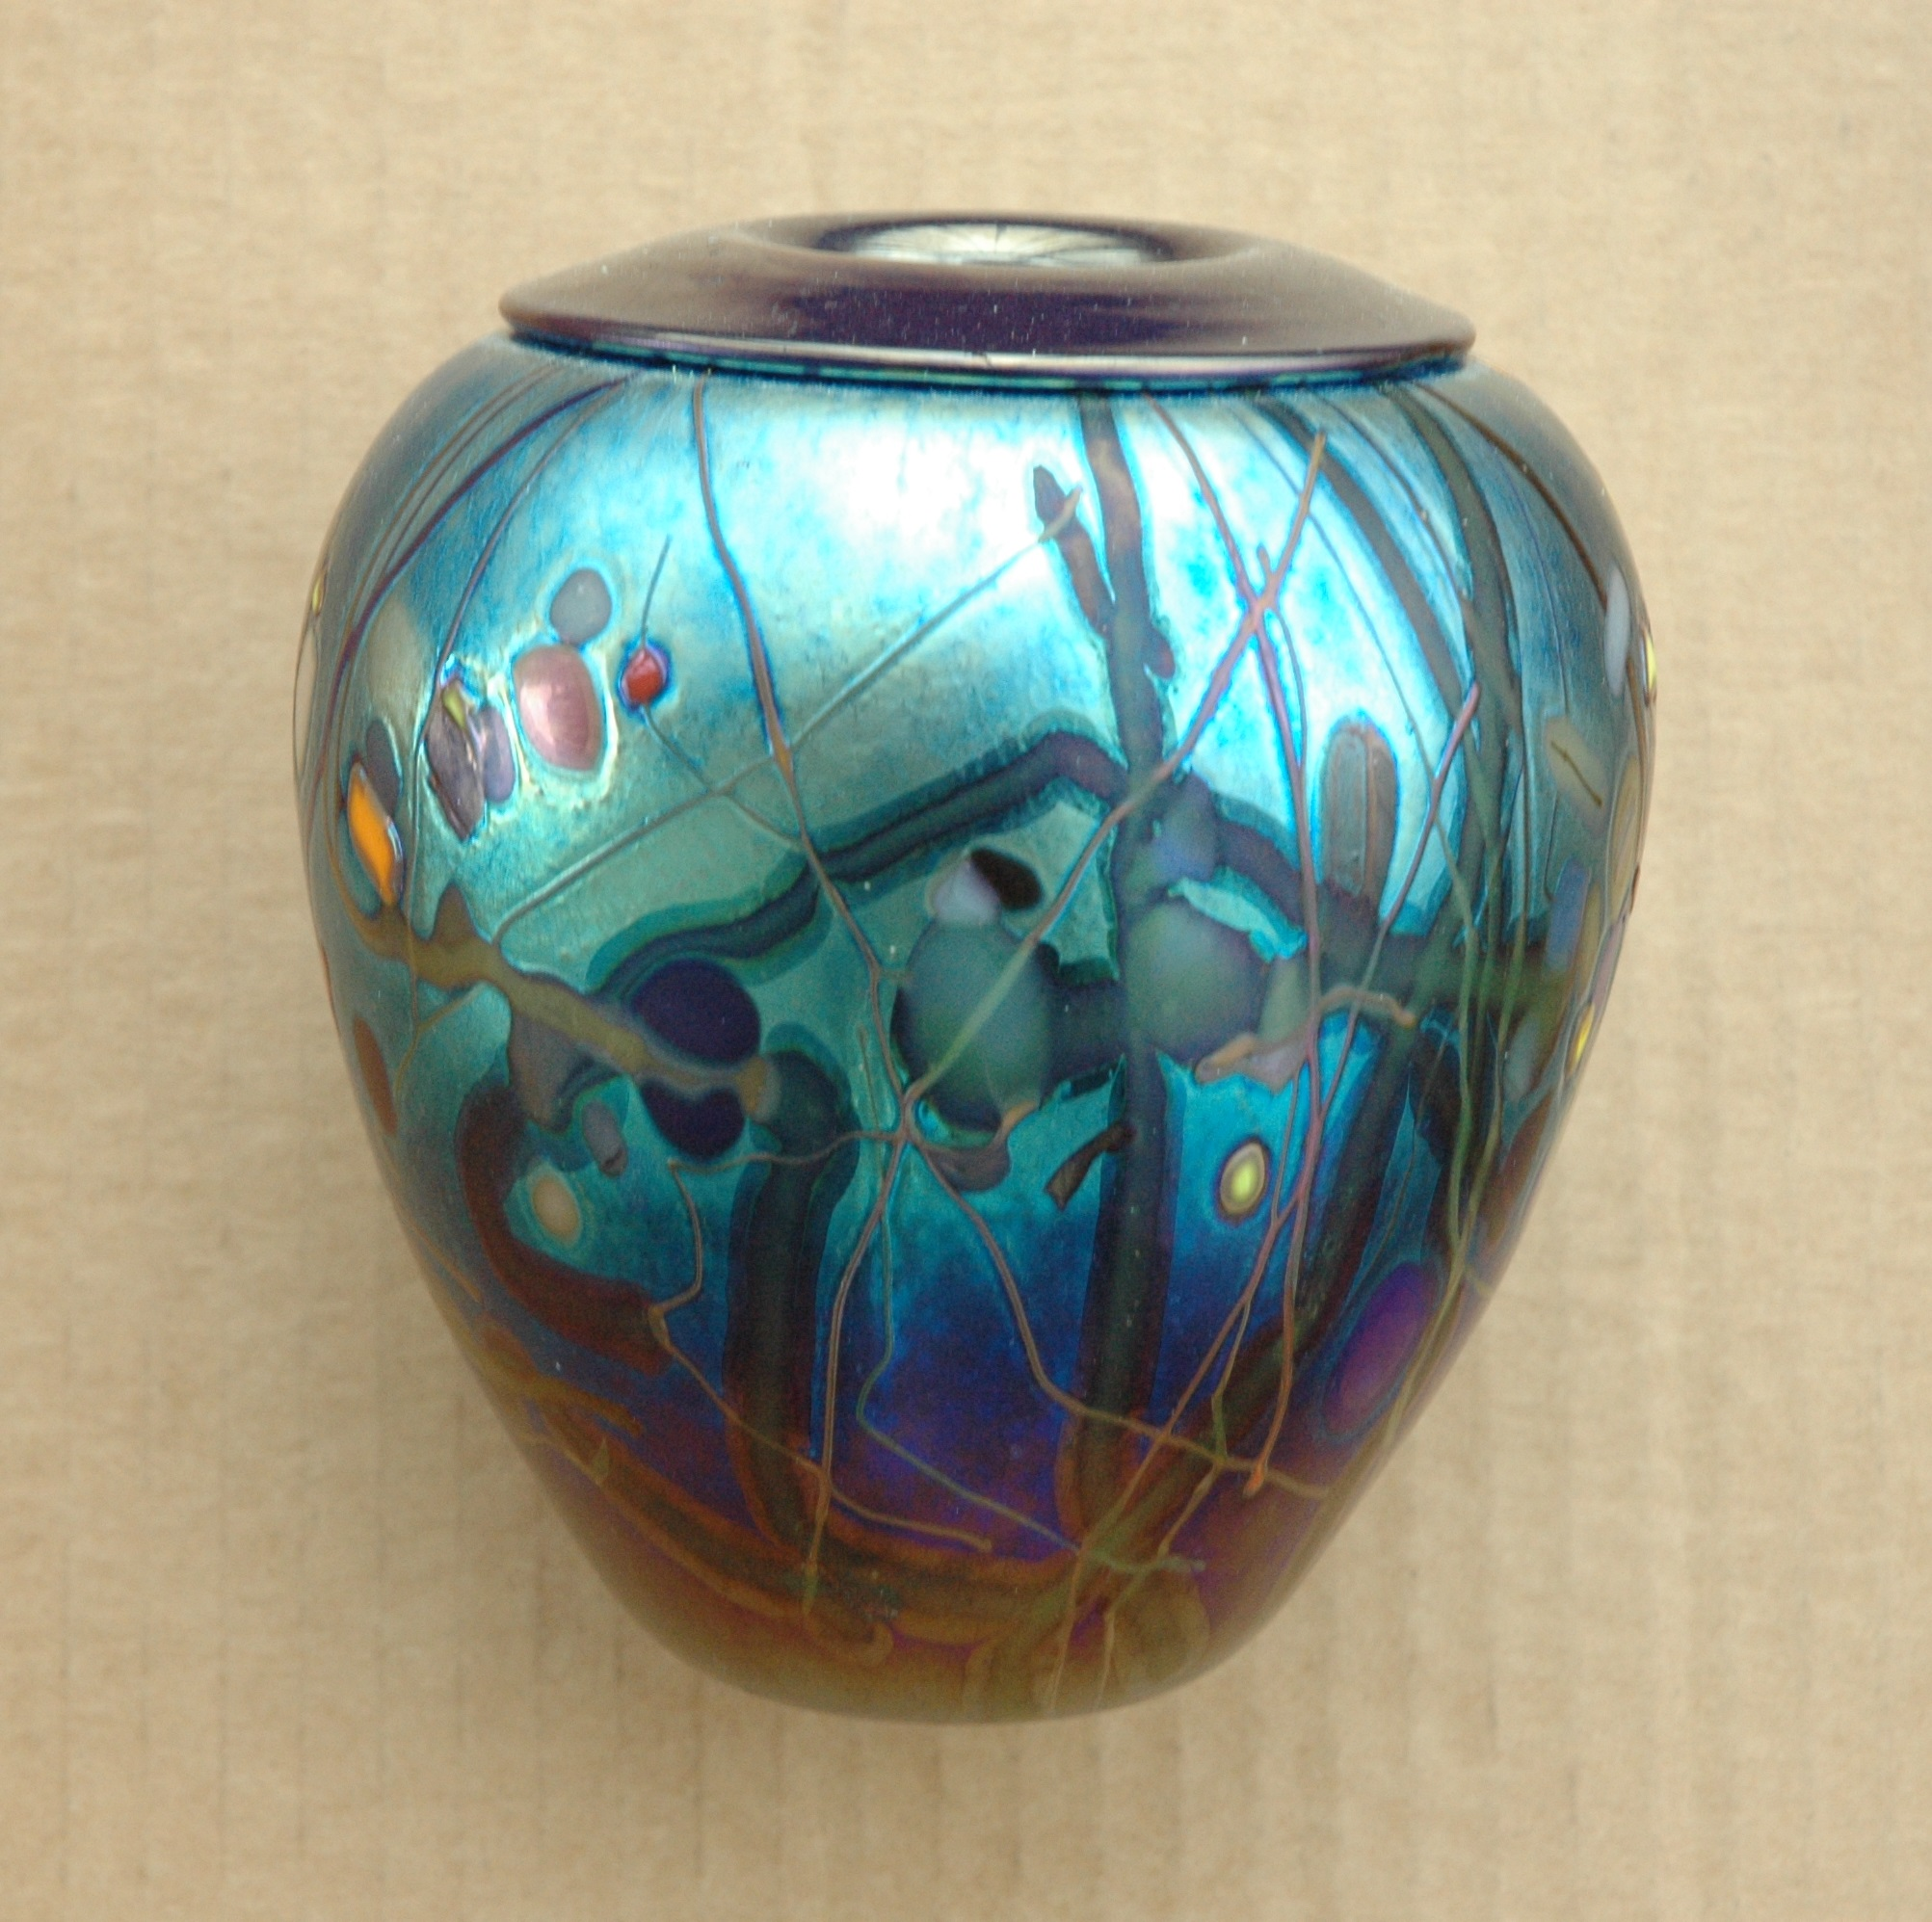
\includegraphics[width=0.25\textwidth]{interp/real_world_obj/vase/vase}}\\
%   \includegraphics[width=0.1\textwidth]{interp/real_world_obj/statue/base_00} & & &
%   \includegraphics[width=0.1\textwidth]{interp/real_world_obj/cup/base_00} & &
%   \includegraphics[width=0.1\textwidth]{interp/real_world_obj/pot/base_00} &
%   \includegraphics[width=0.1\textwidth]{interp/real_world_obj/pot/base_01} & &
%   \includegraphics[width=0.1\textwidth]{interp/real_world_obj/vase/base_00} &
%   \includegraphics[width=0.1\textwidth]{interp/real_world_obj/vase/base_01}\\
%   \multicolumn{3}{c}{(d). statue} & \multicolumn{3}{c}{(e). cup} & 
%   \multicolumn{3}{c}{(g). pot} & \multicolumn{3}{c}{(i). vase} \\
%   \end{tabular}
%   \caption{Material of Real-world objects.}
%   \label{fig:real_data_material}
% \end{table}

From the the decomposition of the material, we can have the property matrix shown in Table~\ref{tab:real_data_prop_list}.
\begin{table}[!htbp]
  \centering
  \begin{tabular}{l*{5}{c}}
  \hline
  \textbf{Property} & Texture & Albedo & Specular & Roughness & Best-suited Algo.\\
  \hline
  status & 0.2 & 0.8 & 0.2 & 0.5 & PS, SL\\
  cup & 0.2 & 0.8 & 0.2 & 0.2 & PS, SL\\
  pot & 0.5 & 0.2, 0.5 & 0.2 & 0.2 & MVS, SL\\
  vase & 0.8 & 0.8, 0.2 & 0.2 & 0.2 & None\\
  \hline
  \end{tabular}
  \caption{Property list for the real-world objects}
  \label{tab:real_data_prop_list}
\end{table}

% In Figure~\ref{fig:test_real_world_obj}, we show the reconstructions of the real-world dataset. Since we don't have the ground truth, no quantitative measures are available, only visual inspection is used. We can show that the qualitative results match the results returned by the mapping.

\begin{figure}[!htbp]
\centering
\begin{tabular}{cc|ccc}
Object & Mapping & ~ & Qualitative results & ~\\
\hline
vase & PS, SL & 
\raisebox{-.5\height}{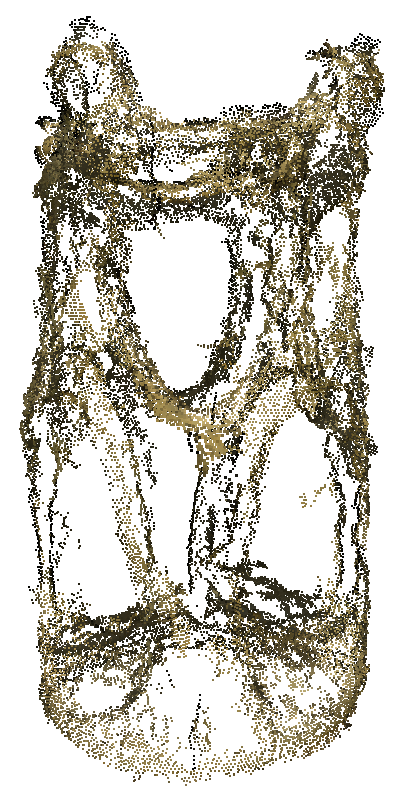
\includegraphics[width=0.2\textwidth]{interp/real_data/statue/statue_mvs_00}}&
\fcolorbox{red}{white}{\raisebox{-.5\height}{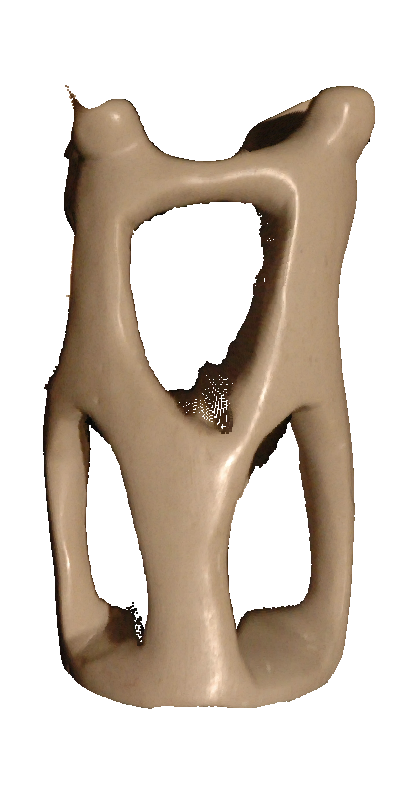
\includegraphics[width=0.2\textwidth]{interp/real_data/statue/statue_ps_00}}}&
\fcolorbox{red}{white}{\raisebox{-.5\height}{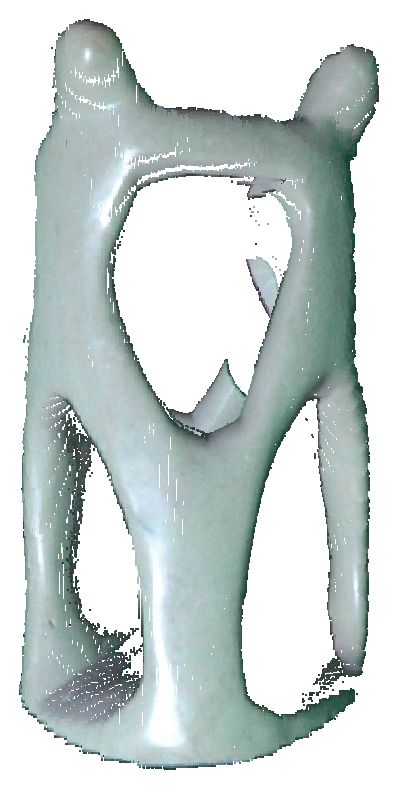
\includegraphics[width=0.2\textwidth]{interp/real_data/statue/statue_sl_00}}}\\
cup & PS, SL &
\raisebox{-.5\height}{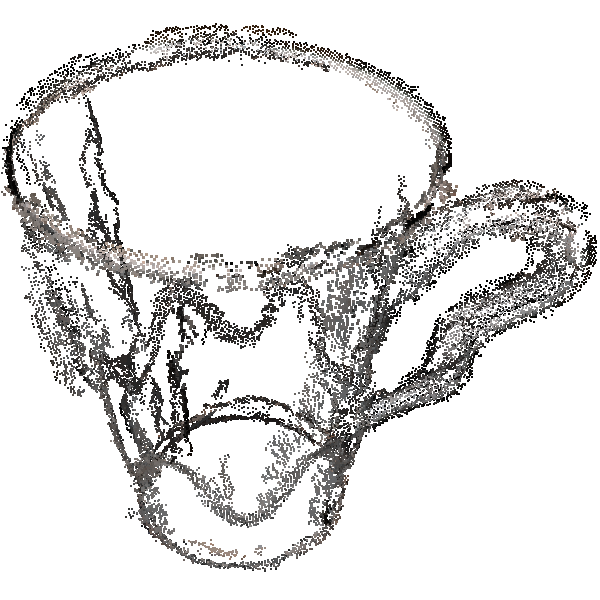
\includegraphics[width=0.2\textwidth]{interp/real_data/cup/cup_mvs_00}}&
\fcolorbox{red}{white}{\raisebox{-.5\height}{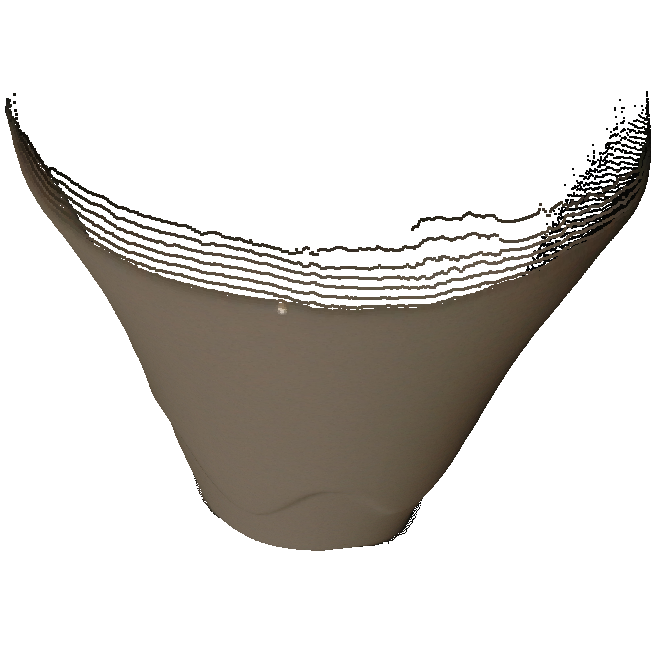
\includegraphics[width=0.2\textwidth]{interp/real_data/cup/cup_ps_00}}}&
\fcolorbox{red}{white}{\raisebox{-.5\height}{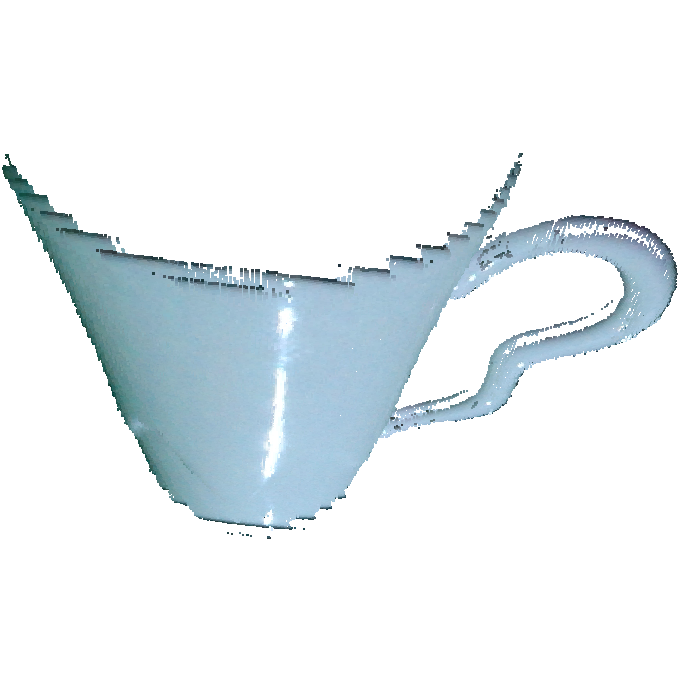
\includegraphics[width=0.2\textwidth]{interp/real_data/cup/cup_sl_00}}}\\
pot & MVS &
\fcolorbox{red}{white}{\raisebox{-.5\height}{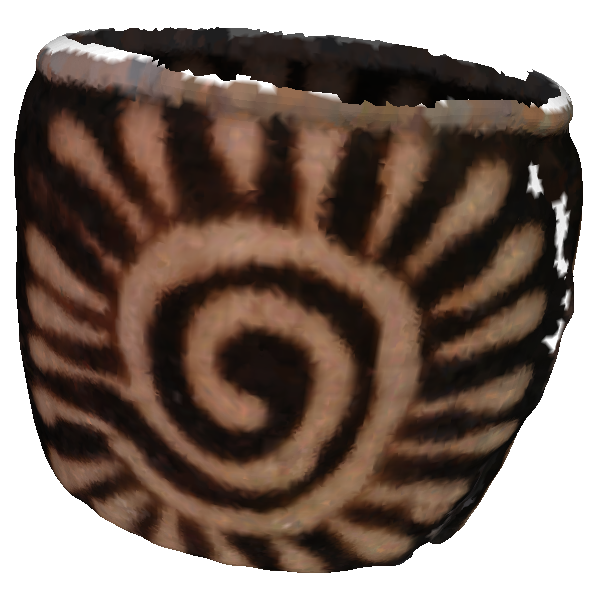
\includegraphics[width=0.2\textwidth]{interp/real_data/pot/pot_mvs_01}}}&
\raisebox{-.5\height}{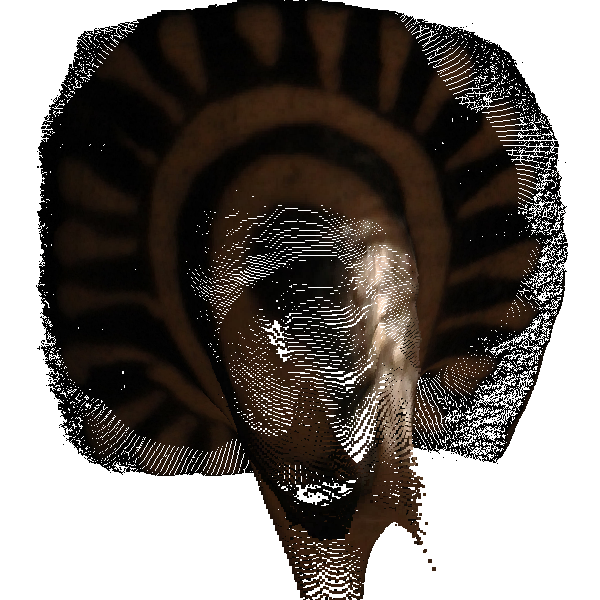
\includegraphics[width=0.2\textwidth]{interp/real_data/pot/pot_ps_00}}&
\raisebox{-.5\height}{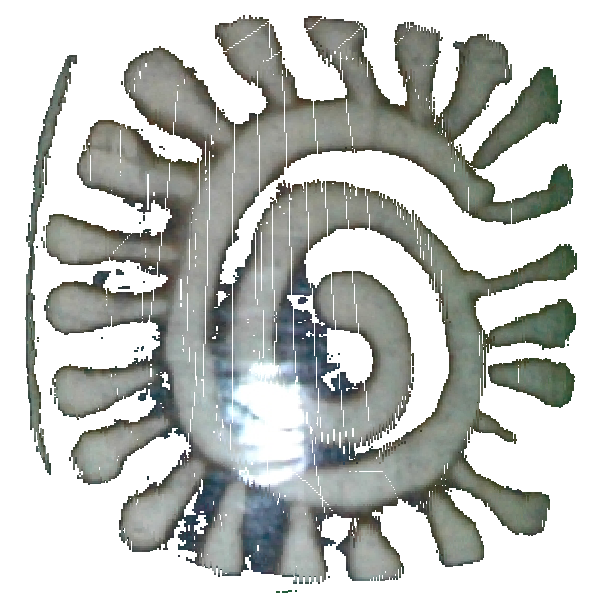
\includegraphics[width=0.2\textwidth]{interp/real_data/pot/pot_sl_00}}\\
vase & MVS &
\fcolorbox{red}{white}{\raisebox{-.5\height}{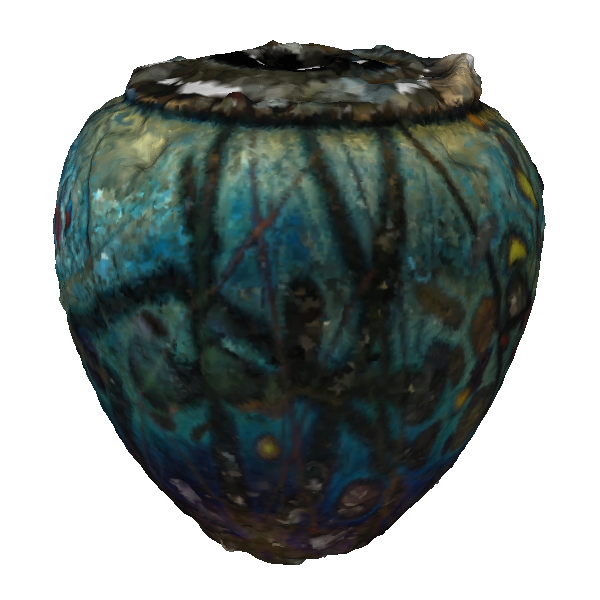
\includegraphics[width=0.2\textwidth]{interp/real_data/vase/vase_mvs_01}}}&
\raisebox{-.5\height}{\includegraphics[width=0.2\textwidth]{interp/real_data/vase/vase_ps_00}}&
\raisebox{-.5\height}{\includegraphics[width=0.2\textwidth]{interp/real_data/vase/vase_sl_00}}\\
\hline
& & PMVS & EPS & GSL\\
\end{tabular}
\caption{The evaluation of the effectiveness of the mapping using real-world object. The well reconstructed object is label by red rectangle.}
\end{figure}

\section{Robustness of Mapping}
Aside from testing whether the description would be correctly mapped to the best algorithm, we should also test given incorrect description, would the mapping return the algorithm that gives less satisfactory results.

As presented in the evaluation steps, we need to give both correct and incorrect description to an object and see if the mapping would give the same mapped algorithm or actually would return difference ones.

\section{Summary}

